%% LyX 2.0.3 created this file.  For more info, see http://www.lyx.org/.
%% Do not edit unless you really know what you are doing.
\documentclass[11pt,english]{report}
\usepackage[T1]{fontenc}
\usepackage[latin9]{inputenc}
\usepackage[a4paper]{geometry}
\geometry{verbose,tmargin=2.6cm,bmargin=3.5cm,lmargin=2.6cm,rmargin=2.6cm}
\usepackage{fancyhdr}
\pagestyle{fancy}
\setlength{\parskip}{\smallskipamount}
\setlength{\parindent}{0pt}
\usepackage{babel}
\usepackage{textcomp}
\usepackage{mathrsfs}
\usepackage{url}
\usepackage{amsmath}
\usepackage{amssymb}
\usepackage{graphicx}
\usepackage{esint}
\usepackage[unicode=true,
 bookmarks=true,bookmarksnumbered=true,bookmarksopen=false,
 breaklinks=true,pdfborder={0 0 0},backref=page,colorlinks=false]
 {hyperref}
\hypersetup{pdftitle={Theoretical quantum mechanics},
 pdfauthor={Andreas V�lklein},
 pdfkeywords={Theoretical quantum mechanics, Physics}}

\makeatletter

%%%%%%%%%%%%%%%%%%%%%%%%%%%%%% LyX specific LaTeX commands.
\providecommand{\LyX}{\texorpdfstring%
  {L\kern-.1667em\lower.25em\hbox{Y}\kern-.125emX\@}
  {LyX}}
\newcommand{\noun}[1]{\textsc{#1}}

\@ifundefined{date}{}{\date{}}
%%%%%%%%%%%%%%%%%%%%%%%%%%%%%% User specified LaTeX commands.
\usepackage{tikz,pgfplots}
%\usepackage{tikz-3dplot}
\usetikzlibrary{matrix,arrows,calc,decorations.pathmorphing,snakes,intersections}
\usepackage{latexsym,stmaryrd,stackrel,array,tabularx,multirow,icomma,braket,polynom,cancel}
\usepackage[explicit]{titlesec}

% Inhaltsverzeichnis
\usepackage{tocloft}
\tocloftpagestyle{fancy}

\renewcommand{\cftchapindent}{1 em}
\renewcommand{\cftchapnumwidth}{1.5 em}

\renewcommand{\cftsecindent}{2.7 em}
\renewcommand{\cftsecnumwidth}{2.5em}

\renewcommand{\cftsubsecindent}{5.2 em}
\renewcommand{\cftsubsecnumwidth}{3.8 em}

\renewcommand{\cftsubsubsecindent}{9 em}
\renewcommand{\cftsubsubsecnumwidth}{4.5 em}

% Mathe-Operatoren
\DeclareMathOperator*{\exsop}{\exists}
\DeclareMathOperator*{\exsgop}{\exists!}
\DeclareMathOperator*{\fallop}{\forall}
\DeclareMathOperator*{\bcupdop}{\dot{\bigcup}}
\DeclareMathOperator*{\bcapdop}{\dot{\bigcap}}

% Rotieren
\newcommand{\Rotate}[1]{
\begin{tikzpicture}
\node[rotate=90] {\ensuremath{#1}};
\end{tikzpicture}
}

%QED-Zeichen (Box)
\newcommand{\qed}{\ensuremath{\Box}}
\newcommand{\qqed}[1][\arabic{chapter}.\arabic{section}\ifnum\arabic{subsection}>0{.\arabic{subsection}}\fi]{\hfill\qed\ensuremath{_{\text{#1}}}}

% Mengen Modulo
\newcommand{\moduloT}[2]{
\mbox{\raisebox{0.6ex}{\ensuremath{\displaystyle #1}}
{\hspace*{-1.5mm}\Large /}
\raisebox{-0.6ex}{\hspace*{-1.5mm}\ensuremath{\displaystyle #2}}
}}

% Links Modulo
\newcommand{\lmoduloT}[2]{
\mbox{\raisebox{-0.6ex}{\ensuremath{\displaystyle #1}}
{\hspace*{-1.5mm}\Large \ensuremath{\backslash}}
\raisebox{0.6ex}{\hspace*{-1.5mm}\ensuremath{\displaystyle #2}}
}}

% F�r Z/2Z, um nicht soviel schreiben zu m�ssen
\newcommand{\modloT}[2]{\moduloT{ \mathbb{#1}}{#2\mathbb{#1}}}

%Die Modulo-Kommandos in klein, f�r die Darstellungen unter Quantoren.
\newcommand{\moduloScriptT}[2]{
\mbox{\raisebox{0.4ex}{\scriptsize\ensuremath{\displaystyle #1}}
{\hspace*{-1.5mm}\footnotesize /}
\raisebox{-0.4ex}{\hspace*{-1.5mm}\scriptsize\ensuremath{\displaystyle #2}}
}}

\newcommand{\lmoduloScriptT}[2]{
\mbox{\raisebox{-0.4ex}{\scriptsize\ensuremath{\displaystyle #1}}
{\hspace*{-1.5mm}\footnotesize \ensuremath{\backslash}}
\raisebox{0.4ex}{\hspace*{-1.5mm}\scriptsize\ensuremath{\displaystyle #2}}
}}

\newcommand{\modloScriptT}[2]{\moduloScriptT{ \mathbb{#1}}{#2\mathbb{#1}}}

% stehendes Winkelzeichen
\newcommand{\winkel}{
\begin{tikzpicture}[scale=0.25]
\draw ({-2+3^(1/2)},0) -- (0,1) -- ({2-3^(1/2)},0);
\draw ($(0,1) + ({cos(235)*0.7},{sin(315)*0.7})$) arc (235:315:0.7);
\end{tikzpicture}}

% Wurzel mit H�kchen
\newcommand{\hsqrt}[2][{}]{\setbox0=\hbox{$\sqrt[#1]{\phantom{|}\!\! #2\hspace*{1pt}}$}\dimen0=\ht0
  \advance\dimen0-0.2\ht0
  \setbox2=\hbox{\vrule height\ht0 depth -\dimen0}
  {\box0\lower0.4pt\box2}}

% alphabetische Aufz�hlung
\newcounter{ale}
\newcommand{\abc}{\stepcounter{ale}\item[\alph{ale})]}
\newenvironment{abclist}{\begin{itemize} \setcounter{ale}{0}}{\end{itemize}}

%klein-r�mische Aufz�hlung
\newcounter{ale2}
\newcommand{\iii}{\stepcounter{ale2}\item[\textnormal{\roman{ale2})}]}
\newenvironment{iiilist}{\begin{itemize} \setcounter{ale2}{0}}{\end{itemize}}

% Damit nicht immer "Kapitel 1" etc. �ber der Kapitel�berschrift steht
\titleformat{\chapter}
  {\huge\bfseries}
  {\textrm{\thechapter} }{0pt}
  {\textrm{#1} \thispagestyle{fancy}
  }

% Neudefinition der Abschnittsmarker f�r die Kopfzeile
\renewcommand\partmark[1]{\markboth{#1}{}}
\renewcommand\chaptermark[1]{\markright{\arabic{chapter} #1}}
\renewcommand\sectionmark[1]{}
\renewcommand\subsectionmark[1]{}

% Kopf- und Fu�zeile
% H�he der Kopfzeile
\setlength{\headheight}{14pt}
% obere Trennlinie
%\renewcommand{\headrulewidth}{0.4pt}
\fancyhf{} %alle Kopf- und Fu�zeilenfelder bereinigen
\fancyhead[L]{\textbf{IK1b - Theoretical QM}} %Kopfzeile links
%\fancyhead[C]{\leftmark} %zentrierte Kopfzeile
\fancyhead[R]{\rightmark} %Kopfzeile rechts
\fancyfoot[C]{\thepage\quad\!\!\!\slash\quad\!\!\!\pageref{END-front}} %Seitenzahl der Front-Matter

\AtBeginDocument{
  \def\labelitemi{\normalfont\bfseries{--}}
  \def\labelitemii{\(\circ\)}
  \def\labelitemiii{\(\triangleright\)}
}

\makeatother

\begin{document}






\global\long\def\norm#1{\left\lVert #1\right\rVert }


\global\long\def\abs#1{\left\lvert #1\right\rvert }


\global\long\def\BRA#1{\Bra{#1}}


\global\long\def\KET#1{\Ket{#1}}


\global\long\def\BraKet#1{\Braket{#1}}


\global\long\def\mins{\text{-}}


\global\long\def\exs{\exsop}


\global\long\def\exsg{\exsgop}


\global\long\def\fall{\fallop}


\global\long\def\bcupd{\bcupdop}


\global\long\def\bcapd{\bcapdop}


\global\long\def\sr#1#2#3{\underset{#3}{\overset{#2}{#1}}}


\global\long\def\dd{\textnormal{d}}


\global\long\def\ii{\textbf{i}}


\global\long\def\modulo#1#2{\moduloT{#1}{#2}}


\global\long\def\lmodulo#1#2{\lmoduloT{#1}{#2}}


\global\long\def\modlo#1#2{\modloT{#1}{#2}}


\global\long\def\moduloScript#1#2{\moduloScriptT{#1}{#2}}


\global\long\def\lmoduloScript#1#2{\lmoduloScriptT{#1}{#2}}


\global\long\def\modloScript#1#2{\modloScriptT{#1}{#2}}


\pagenumbering{roman}


\title{\textbf{\Huge \vspace*{-45mm}}\\
\textbf{\Huge Integrated Course Ib}\\
\textbf{\Huge Theoretical quantum mechanics}}


\author{\textit{\small lecture by}\\
\textit{\noun{\small Dr. Juan-Diego Urbina}}\textit{\small }\\
\textit{\small during the summer semester 2012}\\
\textit{\small revision and layout in \LyX{} by}\\
\textit{\noun{\small Andreas V�lklein}}\\
{\small \vspace*{10mm}}\\
{\small 
\includegraphics[clip,width=15cm]{unir}}\textit{\noun{\small }}\\
{\small \vspace*{3mm}}\\
Last changed: \today}

\maketitle
\fancyhead[R]{License}
\setcounter{page}{2} % sonst gibt es aus irgendeinem Grund zweimal die Seite 1!?!?!?

\vspace*{-15mm}


\subsubsection*{ATTENTION}

This script does \emph{not} replace the lecture.

Therefore it is recommended \emph{strongly} to attend the lecture.

These notes are under constant revision, and the level of rigor is
not uniform.

\vfill{}



\subsubsection*{Copyright Notice}

Copyright � 2012 \noun{Andreas V�lklein}

Permission is granted to copy, distribute and/or modify this document
under the terms of the GNU Free Documentation License, Version 1.3
or any later version published by the Free Software Foundation;

with no Invariant Sections, no Front-Cover Texts, and no Back-Cover
Texts.

A copy of the license is included in the section entitled \textquotedblleft{}GNU
Free Documentation License\textquotedblright{}.


\subsubsection*{Disclaimer of Warranty}

\noun{Unless otherwise mutually agreed to by the parties in writing
and to the extent not prohibited by applicable law, }\textbf{\noun{the
Copyright Holders and any other party, who may distribute the Document
as permitted above,   provide the Document \textquotedblleft{}as is}}\textbf{\textquotedblright{},}\textbf{\noun{
without warranty of any kind}}\noun{, expressed, implied, statutory
or otherwise, including, but not limited to, the implied warranties
of merchantability, fitness for a particular purpose, non-infringement,
the absence of latent or other defects, accuracy, or the absence of
errors, whether or not discoverable.}


\subsubsection*{Limitation of Liability}

\textbf{\noun{In no event}}\noun{ unless required by applicable law
or agreed to in writing }\textbf{\noun{will the Copyright Holders,
or any other party, who may distribute the Document as permitted above,
be liable to you for any damages}}\noun{, including, but not limited
to, any general, special, incidental, consequential, punitive or exemplary
damages, however caused, regardless of the theory of liability, arising
out of or related to this license or any use of or inability to use
the Document, even if they have been advised of the possibility of
such damages.}

\textbf{\noun{In no event will the Copyright Holders'/Distributor's
liability to you}}\noun{, whether in contract, tort (including negligence),
or otherwise, }\textbf{\noun{exceed the amount you paid the Copyright
Holders/Distributor}}\noun{ for the document under this agreement.}


\subsubsection*{Links}

The text of the \textquotedblleft{}GNU Free Documentation License\textquotedblright{}
can also be read on the following site:
\begin{quote}
\url{https://www.gnu.org/licenses/fdl-1.3.en.html}
\end{quote}
A transparent copy of the recent version of this document can be downloaded
from:
\begin{quote}
\url{https://github.com/andiv/IK1b}
\end{quote}
\newpage{}

\fancyhead[R]{Literature}


\subsection*{Literature}
\begin{itemize}
\item \noun{Jun J. Sakurai, Jim Napolitano}: \emph{Modern quantum mechanics},
Addison-Wesley, 2011\\
ISBN: 0-321-50336-8
\item \noun{Leonard I. Schiff}: \emph{Quantum mechanics}, McGraw-Hill, 1968\\
ISBN: 0-07-085643-5
\item Any introductory book on quantum mechanics.
\item \noun{Richard P. Feynman, Robert B. Leighton, Matthew L. Sands}: \emph{Lectures
on physics}
\end{itemize}
{\small \newpage{}}\fancyhead[R]{Table of Contents}
\fancyhead[C]{}

\tableofcontents{}\label{END-front}\newpage{}\pagenumbering{arabic}
\fancyfoot[C]{\thepage\quad\!\!\!\slash\quad\!\!\!\pageref{END}} % Seitenzahl des Hauptteils
\fancyhead[R]{\rightmark}
%\fancyhead[C]{\leftmark}%DATE: Mo 16.04.2012

%\setcounter{chapter}{-1}


\chapter{The Formalism and its interpretation}

As any theory about physical phenomenons, quantum mechanics requires

\begin{iiilist}

\iii kinematical aspects: The (mathematical) space where physical
states are represented.

Example from classical mechanics: points in phase space

\iii the definition of observables: Which quantities can be measured
and how to represent them in the space of states?

Example from classical mechanics: any function $f\left(\vec{r},\vec{p}\right)$

(This is more complicated in quantum mechanics.)

\iii an dynamical law: How do states evolve in \textquotedblleft{}time\textquotedblright{}?

Example from classical mechanics: Hamilton's equations determine $\left(\vec{q}\left(t\right)\!,\,\vec{p}\left(t\right)\right)$
depending on $\left(\vec{q}\left(t_{0}\right)\!,\,\vec{p}\left(t_{0}\right)\right)$.

\end{iiilist}


\section{The kinematical aspects of quantum mechanics}

The \noun{first postulate} says:
\begin{quote}
\textquotedblleft{}The state of a quantum mechanical system is represented
as a normalized vector in a (complex) Hilbert space.\\
Vectors, which differ only by a phase, represent the same state.\textquotedblright{}
\end{quote}
To understand what this means, we introduce some concepts:

\begin{abclist}

\abc \emph{Hilbert space}: A (finite or infinite dimensional) complete
vector space with a positive definite scalar product. Following Dirac,
elements in the Hilbert space $\mathcal{H}$ are called \emph{kets}
and we represent them by $\KET{\psi},\KET{\phi}\in\mathcal{H}$.

For complex numbers $a,b\in\mathbb{C}$ also $a\KET{\psi}+b\KET{\phi}\in\mathcal{H}$
is a element of the Hilbert space.

The sum is associative and the product by scalars is distributive.

\abc \emph{Scalar product}: The operation associating a complex number
to each pair of states
\begin{align*}
\left\langle .,.\right\rangle :\mathcal{H}\times\mathcal{H} & \to\mathbb{C}\\
\left(\KET{\psi},\KET{\phi}\right) & \mapsto\left\langle \psi,\phi\right\rangle 
\end{align*}
with the properties
\begin{align*}
\left\langle \eta,a\phi+b\psi\right\rangle  & =a\left\langle \eta,\phi\right\rangle +b\left\langle \eta,\psi\right\rangle  & \left\langle \psi,\phi\right\rangle  & =\left\langle \phi,\psi\right\rangle ^{*}\\
\left\langle \psi,\psi\right\rangle  & \ge0 & \left\langle \psi,\psi\right\rangle =0 & \quad\Leftrightarrow\quad\ket\psi=0
\end{align*}
for $a,b\in\mathbb{C}$ and $ $$\KET{\phi},\KET{\psi},\KET{\eta}\in\mathcal{H}$
is called the scalar product.

The \emph{norm} of a state $\KET{\psi}$ is then defined as:
\begin{align*}
\norm{\psi}:=\norm{\KET{\psi}} & :=\sqrt{\left\langle \psi,\psi\right\rangle }
\end{align*}
If $\norm{\KET{\psi}}=1$, then $\KET{\psi}$ is said to be \emph{normalized}.

\abc \emph{Phase}: A Complex number $z\in\mathbb{C}$ with unit norm,
that means $zz^{*}=1$. It can be represented via a real number $\alpha\in\mathbb{R}$
as $z=e^{\ii\alpha}$.

The physical state associated with $\KET{\psi}$ and $e^{\ii\alpha}\KET{\psi}$
is \noun{the same}.

\abc C\emph{omplete basis}: A family of kets $\left(\KET{\phi_{i}}\right)_{i\in I\subseteq\mathbb{N}}$
such that for \noun{all} states $\KET{\psi}\in\mathcal{H}$, there
is a family of complex numbers $\left(c_{i}\right)_{i\in I\subseteq\mathbb{N}}$
(depending on $\KET{\psi}$) with:
\begin{align*}
\KET{\psi} & =\sum_{i\in I}c_{i}\KET{\phi_{i}}
\end{align*}
If $\left\langle \phi_{i},\phi_{j}\right\rangle =\delta_{ij}$, then
the basis is \emph{complete} and \emph{orthonormal}.

In the case of an uncountably infinite vector space the basis $\left(\KET q\right)_{q\in\mathbb{R}}$
can be written as a function of a real variable. The representation
of $\KET{\psi}$ then is an infinite sum, that is an integral
\begin{align*}
\KET{\psi} & =\int\psi\left(q\right)\KET q\dd q
\end{align*}
and a complete and orthonormal basis is characterized by $\left\langle q,q'\right\rangle =\delta\left(q-q'\right)$.

\abc \emph{Adjoint}: For each Hilbert space $\mathcal{H}$ there
is another Hilbert space $\mathcal{H}^{*}$ called \emph{dual}, with
elements $\bra f\in\mathcal{H}^{*}$, which are \noun{linear functionals}
acting on $\mathcal{H}$:
\begin{align*}
\BRA f:\mathcal{H} & \to\mathbb{C}\\
\KET{\psi} & \mapsto\BraKet{f|\psi}
\end{align*}
$\BraKet{\psi|\phi}$ is called \emph{bracket}. Riesz theorem says,
that there is a \noun{one to one} correspondence between $\mathcal{H}$
and $\mathcal{H}^{*}$:
\begin{align*}
\fall_{\KET{\psi}\in\mathcal{H}} & \ \exs_{\BRA{\psi}\in\mathcal{H}^{*}}\ \fall_{\KET{\phi}\in\mathcal{H}}\ :\ \BraKet{\psi|\phi}=\left\langle \psi,\phi\right\rangle ,\norm{\BRA{\psi}}=\norm{\KET{\psi}}
\end{align*}
The so associated $\BRA{\psi}$ is the \emph{adjoint} of $\KET{\psi}$,
called \emph{bra}, and we write: 
\begin{align*}
^{\dagger}:\mathcal{H} & \to\mathcal{H}^{*}\\
\KET{\psi} & \mapsto\left(\KET{\psi}\right)^{\dagger}=\BRA{\psi}
\end{align*}
The function $^{\dagger}$ is semilinear, that means for $a,b\in\mathbb{C}$
and $\KET{\psi},\KET{\phi}\in\mathcal{H}$ is:
\begin{align*}
\left(a\KET{\psi}+b\KET{\phi}\right)^{\dagger} & =a^{*}\BRA{\psi}+b^{*}\BRA{\phi}
\end{align*}


\abc \emph{Representation}: Assume that $\left(\KET{\phi_{i}}\right)_{i\in I\subseteq\mathbb{N}}$
(respectively $\left(\KET q\right)_{q\in\mathbb{R}}$) is a complete
orthonormal basis. The ket $\KET{\psi}$ is said to \textquotedblleft{}be
represented\textquotedblright{} in that basis by associating:
\begin{align*}
 & \text{discrete case} &  & \text{continous case}\\
\BRA{\psi} & \mapsto\left(\begin{array}{c}
\BraKet{\phi_{1}|\psi}\\
\BraKet{\phi_{2}|\psi}\\
\vdots
\end{array}\right)\in\mathbb{C}^{\left|I\right|} & \KET{\psi} & \mapsto\BraKet{q|\psi}=:\psi\left(q\right)\\
\BRA{\psi} & \mapsto\left(\begin{array}{c}
\BraKet{\phi_{1}|\psi}^{*}\\
\BraKet{\phi_{2}|\psi}^{*}\\
\vdots
\end{array}\right)\in\mathbb{C}^{\left|I\right|} & \BRA{\psi} & \mapsto\BraKet{q|\psi}^{*}=\psi\left(q\right)^{*}
\end{align*}
This $\psi\left(q\right)$ is the wave function.

\abc \emph{Exterior product}: The object $\KET{\phi}\BRA{\psi}:\mathcal{H}\to\mathcal{H}$
is a linear operator acting on $\KET{\eta}\in\mathcal{H}$ defined
by
\begin{align*}
\left(\KET{\phi}\BRA{\psi}\right)\KET{\eta} & :=\underbrace{\BraKet{\psi\eta}}_{\in\mathbb{C}}\KET{\phi}
\end{align*}
with the adjoint:
\begin{align*}
\left(\KET{\phi}\BRA{\psi}\right)^{\dagger} & :=\KET{\psi}\BRA{\phi}
\end{align*}


Example from linear algebra:
\begin{align*}
\vec{v} & =\left(v_{1},\ldots,v_{n}\right)^{T} & \vec{u} & =\left(u_{1},\ldots,u_{n}\right)^{T}
\end{align*}
\begin{align*}
\vec{v}\,^{T}\vec{u} & =\sum_{i=1}^{n}v_{i}u_{i}\\
\vec{u}\vec{v}\,^{T} & =\left(\begin{array}{ccc}
u_{1}v_{1} & \ldots & u_{1}v_{n}\\
\vdots & \ddots & \vdots\\
u_{n}v_{1} & \ldots & u_{n}v_{n}
\end{array}\right)
\end{align*}


\end{abclist}


\section{Observables and measurements in quantum mechanics}

What can be observed and how measurements affect quantum states is
encoded into the following two \noun{postulates}:
\begin{quote}
\textquotedblleft{}Observables in quantum mechanics are represented
by \noun{linear Hermitian operators} on $\mathcal{H}$.\textquotedblright{}

\textquotedblleft{}The results of a measurement of the physical quantity
represented by an observable can only take values belonging to the
\noun{spectrum} of the observable. Just after measurement, that gives
one of the eigenvalues of the observable, the state belongs to corresponding
eigenspace.\textquotedblleft{}
\end{quote}
\begin{abclist}

\abc $\hat{A}:\mathcal{H}\to\mathcal{H}$ is a \emph{linear }operator
if and only if:
\begin{align*}
\hat{A}\left(a\KET{\psi}+b\KET{\phi}\right) & =a\hat{A}\KET{\psi}+b\hat{A}\KET{\phi}
\end{align*}
For every linear operator $\hat{A}$ there is the identity:
\begin{align*}
\BraKet{\psi|\hat{A}\phi} & =\BraKet{\phi|\hat{A}^{\dagger}\psi}^{*}
\end{align*}
$\hat{A}^{\dagger}$ is called the \emph{adjoint} of $\hat{A}$. If
and only if $\hat{A}=\hat{A}^{\dagger}$ then $\hat{A}$ is called
\noun{Hermitian}\emph{\noun{.}}

\abc The \emph{spectrum} of an operator $\hat{Q}$ is defined by
a set of numbers $Q_{i}$, called \emph{eigenvalues}, that fulfill
the equation:
\begin{align*}
\hat{Q}\KET{Q_{i}} & =Q_{i}\KET{Q_{i}}
\end{align*}


The $\KET{Q_{i}}$ are the corresponding eigenvectors. If there is
more than one eigenvector for the same eigenvalue then the spectrum
is called \emph{degenerated} and the different eigenvectors are denoted
by $\KET{Q_{i}^{\left(d\right)}}$ with $d\in D\subseteq\mathbb{N}$.

Hermitian operators have \noun{real} eigenvalues and \noun{orthogonal}
eigenvectors.

That means, if $\hat{A}=\hat{A}^{\dagger}$, $\hat{A}\KET{a_{i}}=a_{i}\KET{a_{i}}$,
then $a_{i}=a_{i}^{*}$ and $\BraKet{a_{i}|a_{j}}=0$ if $i\not=j$.

If the eigenvectors are normalized, then we can write $\BraKet{a_{i}|a_{j}}=\delta_{ij}$.

%DATE: Do 19.04.2012

\abc The \emph{spectrum decomposition }of a Hermitian operator ($\hat{A}=\hat{A}^{\dagger}$)
with 
\begin{align*}
 & \text{discrete case} &  & \text{continous case}\\
\hat{A}\KET{a_{i}} & =a_{i}\KET{a_{i}} &  & \hat{A}\KET a=a\KET a
\end{align*}
is given by:
\begin{align*}
\hat{A} & =\sum_{i\in I}a_{i}\KET{a_{i}}\BRA{a_{i}} & \hat{A} & =\int a\KET a\BRA a\dd a
\end{align*}
In linear algebra a symmetric matrix $M=M^{T}$ with eigenvalues $m_{i}$
for $i\in\left\{ 1,\ldots,n\right\} $ can be written as:
\begin{align*}
M & =\left(\begin{array}{cccc}
m_{1} & 0 & \ldots & 0\\
0 & m_{2} & \ddots & \vdots\\
\vdots & \ddots & \ddots & 0\\
0 & \ldots & 0 & m_{n}
\end{array}\right)=m_{1}\left(\begin{array}{cccc}
1 & 0 & \ldots & 0\\
0 & 0 & \ddots & \vdots\\
\vdots & \ddots & \ddots & 0\\
0 & \ldots & 0 & 0
\end{array}\right)+\ldots+m_{n}\left(\begin{array}{cccc}
0 & 0 & \ldots & 0\\
0 & \ddots & \ddots & \vdots\\
\vdots & \ddots & 0 & 0\\
0 & \ldots & 0 & 1
\end{array}\right)
\end{align*}


\abc The \emph{unit operator} $\hat{I}$ defined by
\begin{align*}
\fall_{\KET{\phi}\in\mathcal{H}}\ :\ \hat{I}\KET{\phi} & =\KET{\phi}
\end{align*}
can be written as
\begin{align*}
 & \text{discrete case} &  & \text{continous case}\\
\hat{I} & =\sum_{i\in I}\KET{a_{i}}\BRA{a_{i}} & \hat{I} & =\int\KET a\BRA a\dd a
\end{align*}
where $\left(\KET{a_{i}}\right)_{i\in I\subseteq\mathbb{N}}$ (respectively
$\left(\KET a\right)_{a\in\mathbb{R}}$) is a complete orthonormal
basis.

\abc The \emph{projection} of $\KET{\psi}$ along a basis vector
$\KET{a_{i}}$ (respectively $\KET a$) is:
\begin{align*}
\text{discrete} & \text{ case} & \text{continous} & \text{ case}\\
\left(\KET{a_{i}}\BRA{a_{i}}\right)\KET{\psi} & =\BraKet{a_{i}|\psi}\KET{a_{i}} & \left(\KET a\BRA a\right)\KET{\psi} & =\BraKet{a|\psi}\KET a
\end{align*}


\abc The \emph{algebra} of the operators $\hat{Q}_{1}$ and $\hat{Q}_{2}$
is:
\begin{align*}
\left(\hat{Q}_{1}\hat{Q}_{2}\right)\KET{\psi} & :=\hat{Q}_{1}\left(\hat{Q}_{2}\KET{\psi}\right)\not=\left(\hat{Q}_{2}\hat{Q}_{1}\right)\KET{\psi}\\
\left(\hat{Q}_{1}\hat{Q}_{2}\right)^{\dagger} & :=\hat{Q}_{2}^{\dagger}\hat{Q}_{1}^{\dagger}
\end{align*}
The \emph{commutator} is defined by:
\begin{align*}
\left[\hat{Q}_{1},\hat{Q}_{2}\right] & :=\hat{Q}_{1}\hat{Q}_{2}-\hat{Q}_{2}\hat{Q}_{1}
\end{align*}
It is bilinear and has the properties:

\begin{iiilist}

\iii It is antisymmetric:
\begin{align*}
\left[\hat{Q}_{1},\hat{Q}_{2}\right] & =-\left[\hat{Q}_{2},\hat{Q}_{1}\right]
\end{align*}


\iii Jacobi identity:
\begin{align*}
\left[\hat{Q}_{1},\left[\hat{Q}_{2},\hat{Q}_{3}\right]\right]+\left[\hat{Q}_{2},\left[\hat{Q}_{3},\hat{Q}_{1}\right]\right]+\left[\hat{Q}_{3},\left[\hat{Q}_{1},\hat{Q}_{2}\right]\right] & =0
\end{align*}


\iii Leibniz identity:
\begin{align*}
\left[\hat{Q}_{1},\hat{Q}_{2}\hat{Q}_{3}\right]= & \hat{Q}_{2}\left[\hat{Q}_{1},\hat{Q}_{3}\right]+\left[\hat{Q}_{1},\hat{Q}_{2}\right]\hat{Q}_{3}
\end{align*}


\end{iiilist}

Due to these identities the commutator is analogous to the classical
Poisson bracket.

Two observables $\left(\hat{A}=\hat{A}^{\dagger}\!,\,\hat{B}=\hat{B}^{\dagger}\right)$
are called \emph{compatible} if and only if $\left[\hat{A},\hat{B}\right]=0$.

Theorem: If $\hat{A}$ and $\hat{B}$ are compatible then there exists
a basis $\left(\KET{k_{i}}\right)_{i\in I\subseteq\mathbb{N}}$ such
that:
\begin{align*}
\hat{A}\KET{k_{i}} & =a_{i}\KET{k_{i}}\\
\hat{B}\KET{k_{i}} & =b_{i}\KET{k_{i}}
\end{align*}
Therefore the states $\KET{k_{i}}$ have well defined properties $\left(a_{i},b_{i}\right)$.

\abc

\begin{iiilist}

\iii The \emph{matrix representation} of an operator \noun{with respect
to the basis} $\left(\KET{a_{i}}\right)_{i\in\left\{ 1,\ldots,n\right\} }$
(respectively $\left(\KET q\right)_{q\in\mathbb{R}}$) is:
\begin{align*}
 & \qquad\qquad\text{discrete case} &  & \text{continuous case}\\
\hat{Q} & \to\left(\begin{array}{ccc}
\BraKet{a_{1}|\hat{Q}|a_{1}} & \ldots & \BraKet{a_{1}|\hat{Q}|a_{n}}\\
\vdots & \ddots & \vdots\\
\BraKet{a_{n}|\hat{Q}|a_{1}} & \ldots & \BraKet{a_{n}|\hat{Q}|a_{n}}
\end{array}\right)= & \hat{Q} & \to\BraKet{q|\hat{Q}|q'}=Q\left(q,q'\right)\\
 & \quad=\left(\BraKet{a_{i}|\hat{Q}|a_{j}}\right)_{ij}=:Q_{ij}
\end{align*}


\iii The \emph{trace} of $\hat{Q}$ is defined by
\begin{align*}
 & \text{discrete case} &  & \text{continuous case}\\
\text{Tr}\left(\hat{Q}\right) & =\sum_{i=1}^{n}\BraKet{a_{i}|\hat{Q}|a_{i}} & \text{Tr}\left(\hat{Q}\right) & =\int Q\left(q,q\right)\dd q
\end{align*}
ans is independent of the basis.

\end{iiilist}

Therefore the equation
\begin{align*}
\hat{Q}\KET{\psi} & =\KET{\phi}
\end{align*}
can be written in this basis by:

\begin{iiilist}

\iii Multiplying $\BRA{a_{i}}$ from the left: $\BraKet{a_{i}|\hat{Q}|\phi}=\BraKet{a_{i}|\phi}$

\iii Insert an unit operator after $\hat{Q}$:
\begin{align*}
\BraKet{a_{i}|\hat{Q}\hat{I}|\phi} & =\BraKet{a_{i}|\hat{Q}\left(\sum_{j=1}^{n}\KET{a_{j}}\BRA{a_{j}}\right)|\phi}=\sum_{j=1}^{n}\BraKet{a_{i}|\hat{Q}|a_{j}}\BraKet{a_{j}|\phi}=\BraKet{a_{i}|\phi}
\end{align*}
This is the component form of the vector equation:
\begin{align*}
\left(\begin{array}{ccc}
Q_{11} & \ldots & Q_{1n}\\
\vdots &  & \vdots\\
Q_{n1} & \ldots & Q_{nn}
\end{array}\right)\left(\begin{array}{c}
\psi_{1}\\
\vdots\\
\psi_{n}
\end{array}\right) & =\left(\begin{array}{c}
\phi_{1}\\
\vdots\\
\phi_{n}
\end{array}\right)
\end{align*}


\end{iiilist}

The continuous version is
\begin{align*}
\int Q\left(q,q'\right)\psi\left(q'\right)\dd q' & =\phi\left(q\right)
\end{align*}
with $Q\left(q,q'\right):=\BraKet{q|\hat{Q}|q}$, $\psi\left(q'\right)=\BraKet{q'|\psi}$
and $\phi\left(q\right)=\BraKet{q|\phi}$.

\abc Change of basis and unitary transformations.

\begin{iiilist}

\iii An operator $\hat{U}$ is called \emph{unitary} if and only
if $\hat{U}^{T}=\hat{U}^{-1}$.

\iii Unitary transformations (\textquotedblleft{}transformation\textquotedblright{}
is the same as \textquotedblleft{}operator\textquotedblright{}) preserve
scalar products. For $\KET{\psi},\KET{\phi}\in\mathcal{H}$ we define:
\begin{align*}
\KET{\psi'} & :=\hat{U}\KET{\psi} & \KET{\phi'} & :=\hat{U}\KET{\phi}
\end{align*}
Then the scalar product is the same:
\begin{align*}
\BraKet{\psi'|\phi'} & =\BraKet{\psi|\phi}
\end{align*}


\iii Unitary transformations represent changes of the basis.
\begin{align*}
\KET{\psi} & =\hat{I}\KET{\psi}=\left(\sum_{i}\KET{a_{i}}\BRA{a_{i}}\right)\KET{\psi}=\sum_{i\in I}\BraKet{a_{i}|\psi}\KET{a_{i}}\\
\BraKet{b_{i}|\psi} & =\sum_{j\in I}\BraKet{b_{i}|a_{j}}\BraKet{a_{j}|\psi}
\end{align*}
\begin{align*}
\left(\begin{array}{c}
\psi_{1}^{\left(b\right)}\\
\vdots\\
\psi_{N}^{\left(b\right)}
\end{array}\right) & =\mathbb{U}\cdot\left(\begin{array}{c}
\psi_{1}^{\left(a\right)}\\
\vdots\\
\psi_{N}^{\left(a\right)}
\end{array}\right)\\
\left[\mathbb{U}\right]_{ij} & =U_{ij}=\BraKet{b_{i}|a_{j}}
\end{align*}


\iii For operators the transformations are:
\begin{align*}
Q_{ij}^{\left(b\right)} & =\BraKet{b_{i}|\hat{Q}|b_{j}}=\BraKet{b_{i}|\hat{I}\hat{Q}\hat{I}|b_{j}}=\sum_{l,m\in I}\BraKet{b_{i}|a_{l}}\BraKet{a_{l}|\hat{Q}|a_{m}}\BraKet{a_{m}|b_{j}}=\\
 & =\sum_{l,m\in I}U_{il}Q_{lm}^{\left(a\right)}U_{mj}=\sum_{l,m}U_{il}Q_{lm}^{\left(a\right)}\left(U_{jm}\right)^{*}\\
\mathbb{Q}^{\left(b\right)} & =\mathbb{U}\mathbb{Q}^{\left(a\right)}\mathbb{U}^{\dagger}
\end{align*}


\end{iiilist}

%DATE: Di 24.4.12

\abc One can describe functions mapping one operator to another by
their Taylor series:
\begin{align*}
f\left(x\right) & =\sum_{n=0}^{\infty}c_{n}x^{n}\\
c_{n} & =\frac{1}{n!}\partial_{x}^{n}f\left(x\right)\big|_{x=0}\\
f\left(\hat{Q}\right) & :=\sum_{n=0}^{\infty}c_{n}\hat{Q}^{n}
\end{align*}
This is very nice. But this does not work for more than one operator,
if they do not commute.
\begin{align*}
f\left(x,y\right) & =\sum_{n,m}c_{n,m}x^{n}y^{m}\\
f\left(\hat{Q}_{1},\hat{Q}_{2}\right) & \not=\sum_{n,m}c_{n,m}\hat{Q}_{1}^{n}\hat{Q}_{2}^{m}\\
xy & \stackrel{?}{\to}\begin{cases}
\hat{Q}_{1}\hat{Q}_{2}\\
\hat{Q}_{2}\hat{Q}_{1}\\
\frac{1}{2}\left(\hat{Q}_{1}\hat{Q}_{2}+\hat{Q}_{2}\hat{Q}_{1}\right)
\end{cases}
\end{align*}
In a basis of eigenvectors $\KET{q_{i}}$, that means $\hat{Q}\KET{q_{i}}=q_{i}\KET{q_{i}}$,
one can write:
\begin{align*}
 & \text{discrete case} &  & \text{continuous case}\\
f\left(\hat{Q}\right) & =\sum_{i}f\left(q_{i}\right)\KET{q_{i}}\BRA{q_{i}} & f\left(\hat{Q}\right)= & \int f\left(q\right)\KET q\BRA q\dd q
\end{align*}


\abc An operator can also depend on parameters:
\begin{align*}
\mathbb{R}\ni t & \mapsto\hat{A}\left(t\right)\in\text{End}_{\mathbb{C}}\left(\mathcal{H}\right)
\end{align*}
It has all the nice properties, but one has to be careful not to change
the ordering of the operators, if they do not commute:

\begin{align*}
\frac{\dd}{\dd t}\left(\hat{A}\left(t\right)\hat{B}\left(t\right)\right) & =\left(\frac{\dd\hat{A}\left(t\right)}{\dd t}\right)\hat{B}\left(t\right)+\hat{A}\left(t\right)\left(\frac{\dd\hat{B}\left(t\right)}{\dd t}\right)
\end{align*}
\begin{align*}
\frac{\dd\hat{A}\left(t\right)}{\dd t} & =\hat{B}\left(t\right)\quad\Rightarrow\quad\hat{A}\left(t\right)=\int_{0}^{t}\hat{B}\left(t'\right)\dd t'+\hat{A}_{0}
\end{align*}


Extra property: 
\begin{align*}
\frac{\dd}{\dd t}\left(\BraKet{\psi\left(t\right)|\phi\left(t\right)}\right) & =\left(\frac{\dd\BRA{\psi\left(t\right)}}{\dd t}\right)\KET{\phi\left(t\right)}+\BRA{\psi\left(t\right)}\left(\frac{\dd\KET{\phi\left(t\right)}}{\dd t}\right)
\end{align*}


As norm one usually uses:
\begin{align*}
\norm{\hat{A}}^{2} & =\text{Tr}\left(\hat{A}\hat{A}^{\dagger}\right)
\end{align*}


\end{abclist}


\section{What does quantum actually predict?}

Think about classical mechanics:
\begin{align*}
\left(x\left(0\right),p\left(0\right)\right) & \xrightarrow{\text{evolution}}\left(x\left(t\right),p\left(t\right)\right)\to f\left(x\left(t\right),p\left(t\right)\right)\text{ is known}
\end{align*}
So classical mechanics is \noun{deterministic} (the state of a system
is determined by the initial conditions) and \noun{realistic} (the
value you are going to measure already exists before the actual measurement).

Back to quantum mechanics:

The full dynamics is encoded in the postulate:
\begin{quote}
\textquotedblleft{}In each quantum mechanical system there exists
an observable $\hat{H}\!\left(t\right)$, called \emph{Hamiltonian}
which is assumed to be \noun{bounded} from below (and it is a nice
operator). The solution of the equation
\begin{align*}
\ii\hbar\partial_{t}\hat{U}\left(t,t_{0}\right) & =\hat{H}\left(t\right)\hat{U}\left(t,t_{0}\right) & \hat{U}\left(t_{0},t_{0}\right) & =\hat{I} &  & \text{for }t>t_{0}
\end{align*}
is an unitary operator $\hat{U}$, called \noun{time evolution operator}.
The time evolution of an initial state $\KET{\psi\left(t_{0}\right)}$
is given by $\KET{\psi\left(t\right)}=\hat{U}\left(t,t_{0}\right)\KET{\psi\left(t_{0}\right)}$.\textquotedblright{}
\end{quote}
Comments:

\begin{abclist}

\abc If $\partial_{t}\hat{H}\left(t\right)=0$, the one can directly
solve the Schr�dinger equation:
\begin{align}
\hat{U}\left(t,t_{0}\right) & =e^{\frac{-\ii}{\hbar}\hat{H}\cdot\left(t-t_{0}\right)} &  & \text{for }t>t_{0}\label{eq:SchroedingerOperator}
\end{align}
\abc $\hat{U}$ has a \noun{semigroup} property:
\begin{align*}
\hat{U}\left(t,t'\right)\hat{U}\left(t',t_{0}\right) & =\hat{U}\left(t,t_{0}\right) &  & t>t'>t_{0}
\end{align*}
Semigroup means:
\begin{align*}
\hat{U}\left(t,t_{0}\right)^{-1} & =\hat{U}\left(t,t_{0}\right)^{\dagger}\not=\hat{U}\left(t_{0},t\right)
\end{align*}


\abc Constructing $\hat{H}\left(t\right)$ is the main step to define
a quantum mechanical system, at the end it relies on experimental
verification.

\abc The formal solution of \eqref{eq:SchroedingerOperator} is found
by iteration:
\begin{align*}
\hat{U}\left(t,t_{0}\right) & =\hat{I}-\frac{\ii}{\hbar}\int_{t_{0}}^{t}\hat{H}\left(t'\right)\hat{U}\left(t',t_{0}\right)\dd t' &  & t>t'\\
 & =\hat{I}-\frac{\ii}{\hbar}\int_{t_{0}}^{t}\hat{H}\left(t'\right)\left(\hat{I}-\frac{\ii}{\hbar}\int_{t_{0}}^{t}\hat{H}\left(t''\right)\hat{U}\left(t'',t_{0}\right)\dd t''\right)\dd t'=\\
 & =\hat{I}-\frac{\ii}{\hbar}\int_{t_{0}}^{t}\hat{H}\left(t'\right)\dd t'+\left(\frac{\mins\ii}{\hbar}\right)^{2}\int_{t_{0}}^{t}\int_{t_{0}}^{t'}\hat{H}\left(t'\right)\hat{H}\left(t''\right)\hat{U}\left(t'',t_{0}\right)\dd t''\dd t'=\\
 & =\tau e^{\frac{\mins\ii}{\hbar}\int_{t_{0}}^{t}\hat{H}\left(t'\right)\dd t'}
\end{align*}
$\tau$ is the \noun{time ordering operator}.
\begin{align*}
\tau\left(\hat{H}\left(t\right)\hat{H}\left(t'\right)\right) & =\begin{cases}
\hat{H}\left(t\right)\hat{H}\left(t'\right) & t>t'\\
\hat{H}\left(t'\right)\hat{H}\left(t\right) & t<t'
\end{cases}
\end{align*}


\abc Stationary states: Assume $\partial_{t}\hat{H}\left(t\right)=0$,
then the eigenstates of $\hat{H}$ are defined by the time-independent
Schr�dinger equation:
\begin{align*}
\hat{H}\KET{e_{n}} & =e_{n}\KET{e_{n}}
\end{align*}
Their time evolution is:
\begin{align*}
\KET{e_{n}\left(t\right)} & =e^{\mins\frac{\ii}{\hbar}\hat{H}t}\KET{e_{n}}=\underbrace{e^{\mins\frac{\ii e_{n}}{\hbar}t}}_{\text{phase}}\KET{e_{n}}=e^{\mins\ii\omega_{n}t}\KET{e_{n}}
\end{align*}
 For an arbitrary initial state $\KET{\psi\left(t_{0}\right)}$ we
can calculate the final state:
\begin{align*}
\KET{\psi\left(t\right)} & =e^{\mins\frac{\ii}{\hbar}\hat{H}\cdot\left(t-t_{0}\right)}\KET{\psi\left(t_{0}\right)}=e^{\mins\frac{\ii}{\hbar}\hat{H}\cdot\left(t-t_{0}\right)}\hat{I}\KET{\psi\left(t_{0}\right)}=\\
 & =\sum_{n=0}^{\infty}\BraKet{e_{n}|\psi\left(t_{0}\right)}e^{\mins\ii\omega_{n}\cdot\left(t-t_{0}\right)}\KET{e_{n}}
\end{align*}


\abc Instead of finding $\hat{U}$ we can solve the \noun{Schr�dinger
equation} directly for $\KET{\psi\left(t\right)}$:
\begin{align*}
\ii\hbar\partial_{t}\KET{\psi\left(t\right)} & =\hat{H}\left(t\right)\KET{\psi\left(t\right)}\\
\KET{\psi\left(t=t_{0}\right)} & =\KET{\psi\left(t_{0}\right)}
\end{align*}


\end{abclist}


\section{The probabilistic interpretation of quantum mechanics (Born's rule)}
\begin{quote}
\textquotedblleft{}If the states of a system at time $t$ is given
by the normalized state $\KET{\psi\left(t\right)}$, then the \noun{probability}
to get the outcome $a_{i}$ when the observable $\hat{A}$ is measured
is given by:\textquotedblright{}
\begin{align*}
 & \text{discrete case} &  & \text{continuous case}\\
P\left(a_{i},t\right) & =\abs{\BraKet{a_{i}|\psi\left(t\right)}}^{2} & P\left(q,t\right) & =\abs{\BraKet{q|\psi\left(t\right)}}^{2}\dd q
\end{align*}

\end{quote}
\begin{abclist}

\abc
\begin{align*}
 & \text{discrete case} &  & \text{continuous case}\\
\sum_{i}P\left(a_{i},t\right) & =1 & \int P\left(q,t\right)\dd q & =1
\end{align*}
$\BraKet{a_{i}|\psi\left(t\right)}$ is called probability Amplitude,
$P\left(q,t\right)$ is the density of probability and the probability
to obtain an outcome between $q$ and $q+\dd q$ is $\abs{\BraKet{q|\psi\left(t\right)}}^{2}$.\\
\abc The expectation value is given by:
\begin{align*}
\overline{A} & :=\sum_{i}a_{i}P\left(a_{i},t\right)=\sum_{i}a_{i}\abs{\BraKet{a_{i}|\psi\left(t\right)}}^{2}=\sum_{i}a_{i}\BraKet{a_{i}|\psi\left(t\right)}\cdot\BraKet{a_{i}|\psi\left(t\right)}^{*}=\\
 & =\sum_{i}a_{i}\BraKet{\psi\left(t\right)|a_{i}}\cdot\BraKet{a_{i}|\psi\left(t\right)}=\BRA{\psi\left(t\right)}\left(\sum_{i}a_{i}\KET{a_{i}}\cdot\BRA{a_{i}}\right)\KET{\psi\left(t\right)}=\\
 & =\BraKet{\psi\left(t\right)|\hat{A}|\psi\left(t\right)}=:\left\langle \hat{A}\right\rangle 
\end{align*}
%DATE: Do 26.4.2012
\begin{align*}
\text{Var}\hat{A} & =\left\langle \hat{A}^{2}\right\rangle -\left(\left\langle \hat{A}\right\rangle \right)^{2}=\BraKet{\psi\left(t\right)|\hat{A}^{2}|\psi}-\BraKet{\psi\left(t\right)|\hat{A}|\psi\left(t\right)}^{2}=\\
 & =\left\langle \left(\hat{A}-\hat{I}\left\langle \hat{A}\right\rangle \right)^{2}\right\rangle =\sum\left(a_{i}-\overline{a}_{i}\right)^{2}P\left(a_{i},t\right)=\left(\Delta\hat{A}\right)^{2}
\end{align*}
The only case, one gets
\begin{align*}
\left\langle \left(\hat{A}-\left\langle \hat{A}\right\rangle \right)^{2}\right\rangle  & =0
\end{align*}
is, if $\KET{\psi\left(t\right)}=\KET{a_{i}}$.

\noindent \begin{center}
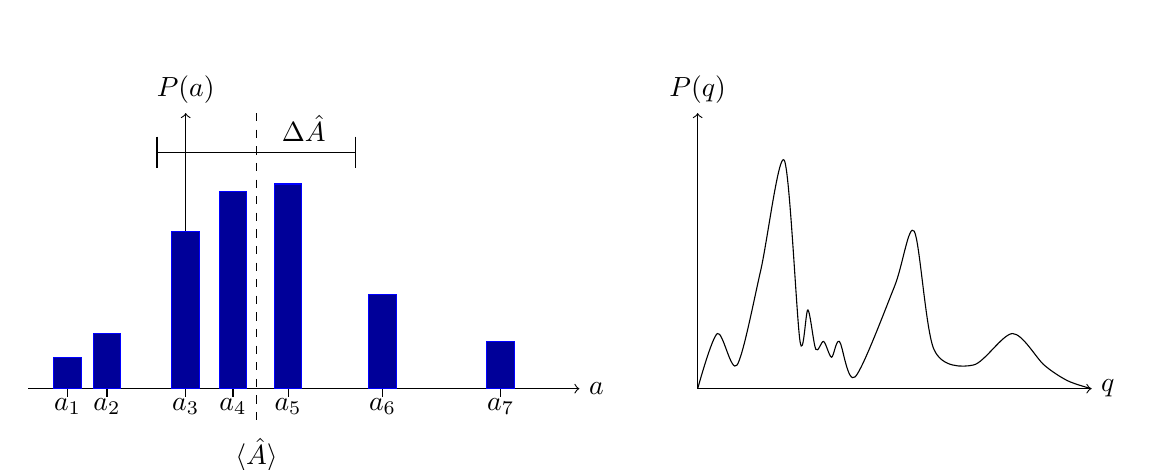
\begin{tikzpicture}
  \draw[->] (-2,0) -- (5,0) node[right] {$a$};
  \draw[->] (0,0) -- (0,3.5) node[above] {$P(a)$};
  \foreach \n/\x in {1/-1.5,2/-1,3/0,4/0.6,5/1.3,6/2.5,7/4}
    \draw (\x,0.1) -- node[below]{$a_\n$} (\x,-0.1);
  \draw[draw=blue,fill=blue!60!black] plot[ybar] coordinates{(-1.5,0.4) (-1,0.7) (0,2) (0.6,2.5) (1.3,2.6) (2.5,1.2) (4,0.6)};
  \draw[dashed] (0.898,3.5) --  (0.898,-0.5) node[below]{$\langle\hat{A}\rangle$};
  \draw (-0.364,3) +(0,0.2) -- +(0,-0.2) +(0,0) -- (2.160,3) +(0,0.2) -- +(0,-0.2);
  \node at (1.5,3.3) {$\Delta \hat{A}$};
 \begin{scope}[xshift=185]
   \draw[->] (0,0) -- (5,0) node[right] {$q$};
   \draw[->] (0,0) -- (0,3.5) node[above] {$P(q)$};
   \draw plot[smooth] coordinates{(0,0) (0.25,0.7) (0.5,0.3) (0.8,1.5) (1.1,2.9) (1.3,0.6) (1.4,1) (1.5,0.5) (1.6,0.6) (1.7,0.4) (1.8,0.6) (2,0.15) (2.5,1.3) (2.75,2) (3,0.5) (3.5,0.3) (4,0.7) (4.4,0.3) (4.7,0.1) (5,0)};
 \end{scope}
\end{tikzpicture} 
\par\end{center}

\abc Consider the eigenstates of the Hamiltonian:
\begin{align*}
\hat{H}\KET{e_{n}} & =e_{n}\KET{e_{n}}
\end{align*}
If at $t=0$ the state is $\KET{e_{n}}$, then the time evolution
is very simple:
\begin{align*}
\KET{e_{n}\left(t\right)} & =e^{-\ii\omega_{n}t}\KET{e_{n}}\\
\Rightarrow\quad\BraKet{e_{n}\left(t\right)|\hat{A}|e_{n}\left(t\right)} & =\BraKet{e_{n}|\hat{A}|e_{n}}\\
\partial_{t}\left\langle \hat{A}\right\rangle  & =0
\end{align*}
\abc Define $\KET{\eta}=N\left(\KET{\psi}+\KET{\phi}\right)$. What
is the probability $P_{\eta}\left(a_{i}\right)$?
\begin{align*}
\abs{\BraKet{a_{i}|\eta}}^{2} & =N^{2}\abs{\BraKet{a_{i}|\psi}+\BraKet{a_{i}|\phi}}^{2}=\\
 & =N^{2}\left(\abs{\BraKet{a_{i}|\psi}}^{2}+\abs{\BraKet{a_{i}|\phi}}^{2}+2\text{Re}\left(\BraKet{a_{i}|\psi}\BraKet{a_{i}|\phi}^{*}\right)\right)=\\
 & =N^{2}\left(P_{\psi}\left(a_{i}\right)+P_{\phi}\left(a_{i}\right)+\text{something}\right)
\end{align*}
Therefore it is not enough to know the probabilities, one also has
to know the phase of the states.

\end{abclist}


\section{``Quantization'':\protect \\
Introducing the ``fundamental'' or basic observables}


\subsection{General approach}

Historically, it all started with the Hydrogen atom. (In this system
the Hilbert space $\mathcal{H}$ is infinite-dimensional.) It is called
``canonical'' quantization.

\begin{iiilist}

\iii $\dim\mathcal{H}=\infty$ means, there can be discrete as well
as continuous eigenvalues.

\iii Every quantum mechanical observable is a function of two basic
observables, the position operator $\hat{q}_{\alpha}$ and the momentum
operator $\hat{p}_{\alpha}$, satisfying:
\begin{align*}
\left[\hat{q}_{\alpha},\hat{p}_{\beta}\right] & =\ii\hbar\delta_{\alpha\beta}\hat{I} & \left[\hat{q}_{\alpha},\hat{q}_{\beta}\right] & =0=\left[\hat{p}_{\alpha},\hat{p}_{\beta}\right]
\end{align*}
Therefore you can define an eigenbasis $\KET{\vec{q}}$ with:
\begin{align*}
\hat{q}_{\alpha}\KET{\vec{q}} & =q_{\alpha}\KET{\vec{q}} & \hat{p}_{\alpha}\KET{\vec{p}} & =p_{\alpha}\KET{\vec{p}} & q_{\alpha},p_{\alpha} & \in\mathbb{R}
\end{align*}
\begin{align*}
\BraKet{\vec{q}|\vec{q}\,'} & =\delta\left(\vec{q}-\vec{q}\,'\right) & \BraKet{\vec{p}|\vec{p}\,'} & =\delta\left(\vec{p}-\vec{p}\,'\right)
\end{align*}
\iii The Hamiltonian operator is given in terms of the classical
Hamiltonian
\begin{align*}
H\left(\vec{q},\vec{p}\right) & =\left(\frac{1}{2m}\sum_{\alpha}p_{\alpha}^{2}\right)+V\left(\vec{q}\right)
\end{align*}
as:
\begin{align*}
\hat{H} & =H\left(\hat{q}_{\alpha},\hat{p}_{\alpha}\right)=\left(\frac{1}{2m}\sum_{\alpha}\hat{p}_{\alpha}^{2}\right)+V\left(\hat{q}_{\alpha}\right)
\end{align*}
 This works \noun{only} in Cartesian coordinates! In other coordinates
the product $pq$ occurs in $H$, but how to quantize $qp$? The operators
do not commute: $\hat{q}\hat{p}\not=\hat{p}\hat{q}$

For a magnetic field with vector potential $\vec{A}\left(\vec{q}\right)$
the Hamiltonian is
\begin{align*}
H & =\frac{1}{2m}\left(\vec{p}+\frac{e}{c}\vec{A}\left(\vec{q}\right)\right)^{2}
\end{align*}
and also depends on products of $\vec{p}$ and $\vec{q}$.
\begin{align*}
\hat{H} & =\sum_{n}e_{n}\KET{e_{n}}\BRA{e_{n}}+\int_{\Omega}e\left(\kappa\right)\KET{e\left(\kappa\right)}\BRA{e\left(\kappa\right)}\dd k
\end{align*}
\begin{align*}
\BraKet{e_{n}|e_{n'}} & =\delta_{n,n'} &  & \text{bounded}\\
\BraKet{e\left(\kappa\right)|e\left(\kappa'\right)} & =\delta\left(\kappa-\kappa'\right) &  & \text{scattering}
\end{align*}


A typical effective potential is:

\noindent \begin{center}
\begin{tikzpicture}[domain=0.5:4,samples=40,xscale=2]
  \draw[->] (-0.2,0) -- (4.2,0) node[right] {$q$};
  \draw[->] (0,-2.2) -- (0,4.2) node[above] {$V_{\text{eff}}(q)$};
  \draw (-0.1,2) node[left]{$E_{\text{scattering}}$} -- (4,2);
  \draw (-0.1,-0.5) node[left]{$E_{\text{bounded}}$} -- (4,-0.5);
  \draw[smooth] plot (\x,{(1/\x^2-3)/\x^2});
  \draw[very thick] (0.595,-0.5) -- (2.376,-0.5);
  \draw[dashed, very thick] (0.595,-0.5) -- (0.595,0) (2.376,-0.5) -- (2.376,0);
  \draw[very thick] (0.529883,2) -- (4,2);
%  \draw[dashed, very thick] (0.529883,2) -- (0.595,0);
\end{tikzpicture} 
\par\end{center}

\iii The representations of a state $\ket\psi$ in the position or
momentum eigenstates are called \noun{wavefunctions}. This means:
\begin{align*}
\KET{\psi} & =\int\underbrace{\BraKet{\vec{q}|\psi}}_{=\psi\left(\vec{q}\right)}\KET{\vec{q}}\dd\vec{q} & \KET{\psi} & =\int\underbrace{\BraKet{\vec{p}|\psi}}_{=\tilde{\psi}\left(\vec{p}\right)}\KET{\vec{p}}\dd\vec{p}
\end{align*}
Born's rule says, that $\abs{\psi\left(\vec{q}\right)}^{2}\dd\vec{q}$
is the probability to find the particle between $\vec{q}$ and $\vec{q}+\left(\dd q_{1},\dd q_{2},\ldots\right)$
and $\abs{\tilde{\psi}\left(\vec{p}\right)}^{2}\dd\vec{p}$ is the
probability to find the particle between $\vec{p}$ and $\vec{p}+\left(\dd p_{1},\dd p_{2},\ldots\right)$.

\end{iiilist}


\subsection{Algebraic properties of $\hat{q}$ and $\hat{p}$}

Consider the following commutators:
\begin{align*}
\left[\hat{q}_{\alpha},\hat{p}_{\beta}^{2}\right] & =\hat{p}_{\beta}\left[\hat{q}_{\alpha},\hat{p}_{\beta}\right]+\left[\hat{q}_{\alpha},\hat{p}_{\beta}\right]\hat{p}_{\beta}=2\ii\hbar\delta_{\alpha\beta}\hat{p}_{\beta}\\
\left[\hat{q}_{\alpha},\hat{p}_{\beta}^{3}\right] & =\hat{p}_{\beta}^{2}\left[\hat{q}_{\alpha},\hat{p}_{\beta}\right]+\hat{p}_{\beta}\left[\hat{q}_{\alpha},\hat{p}_{\beta}\right]\hat{p}_{\beta}+\left[\hat{q}_{\alpha},\hat{p}_{\beta}\right]\hat{p}_{\beta}^{2}=3\ii\hbar\delta_{\alpha\beta}\hat{p}_{\beta}^{2}\\
\vdots\ \ \\
\left[\hat{q}_{\alpha},\hat{p}_{\beta}^{n}\right] & =\sum_{k=1}^{n}\hat{p}_{\beta}^{n-k}\left[\hat{q}_{\alpha},\hat{p}_{\beta}\right]\hat{p}_{\beta}^{k-1}=n\ii\hbar\delta_{\alpha\beta}\hat{p}_{\beta}^{n-1}
\end{align*}
Since every analytic function can be represented by its Taylor series,
one gets:
\begin{align*}
\left[\hat{q}_{\alpha},f\left(\hat{p}_{\beta}\right)\right] & =\ii\hbar\delta_{\alpha\beta}\partial_{x}f\left(x\right)\big|_{x=\hat{p}_{\beta}}=:\ii\hbar\delta_{\alpha\beta}\partial_{\hat{p}_{\beta}}f\left(\hat{p}_{\beta}\right)\\
\left[\hat{p}_{\alpha},f\left(\hat{q}_{\beta}\right)\right] & =-\ii\hbar\delta_{\alpha\beta}\partial_{\hat{q}_{\beta}}f\left(\hat{q}_{\beta}\right)
\end{align*}
One can show:
\begin{align*}
\hat{q}e^{-\frac{\ii}{\hbar}\hat{p}q_{0}}\KET q & =\left(q+q_{0}\right)\KET{q+q_{0}}
\end{align*}
This follows, because $e^{-\frac{\ii}{\hbar}\hat{p}q_{0}}\KET q$
is an eigenstate of $\hat{q}$ with eigenvalue $q+q_{0}$ and therefore:
\begin{align*}
e^{-\frac{\ii}{\hbar}\hat{p}q_{0}}\KET q & =\KET{q+q_{0}}
\end{align*}
%DATE: Do 3.5.2012

One can also show:
\begin{align*}
e^{\frac{\ii}{\hbar}\hat{q}p_{0}}\KET p & =\KET{p+p_{0}}
\end{align*}
This is similar to:
\begin{align*}
e^{-\frac{\ii}{\hbar}\hat{H}t}\KET{\psi\left(t_{0}\right)} & =\KET{\psi\left(t_{0}+t\right)}
\end{align*}



\subsection{The Schr�dinger equation in position and momentum representation}

Consider the Hamiltonian:
\begin{align*}
\hat{H} & =\frac{1}{2m}\hat{p}^{2}+V\left(\hat{q}\right)
\end{align*}
I want to ``represent'':
\begin{align*}
\hat{H}\KET{e_{n}} & =e_{n}\KET{e_{n}}\\
\hat{H}\KET e & =e\KET e
\end{align*}
For position representation, we apply $\BRA q$ to the equation, use
the definitions $\psi_{n}\left(q\right):=\BraKet{q|e_{n}}$ and $\tilde{\psi}_{n}\left(p\right):=\BraKet{p|e_{n}}$,
and multiply with the unit operator $\hat{I}=\int\KET p\BRA p\dd p$
to get:
\begin{align*}
\frac{1}{2m}\BraKet{q|\hat{p}^{2}\cdot\hat{I}|e_{n}}+V\left(q\right)\BraKet{q|e_{n}} & =e_{n}\BraKet{q|e_{n}}\\
\frac{1}{2m}\int p^{2}\BraKet{q|p}\tilde{\psi}_{n}\left(p\right)\dd p+V\left(q\right)\psi_{n}\left(q\right) & =e_{n}\psi_{n}\left(q\right)
\end{align*}
In general one gets:
\begin{align*}
\BraKet{q|f\left(\hat{p}\right)|\psi} & =f\left(-\hbar\partial_{q}\right)\psi\left(q\right)
\end{align*}
The recipe is:
\begin{align*}
\hat{p} & \mapsto-\ii\hbar\partial_{q} &  & \text{one dimension}\\
\hat{p} & \mapsto-\ii\hbar\vec{\nabla} &  & \text{three dimensions}
\end{align*}
In three dimensions this is:
\begin{align*}
\text{discrete case} &  & \text{continuous case}\\
\left(-\frac{\hbar^{2}}{2m}\nabla^{2}+V\left(\vec{q}\right)\right)\psi_{n}\left(\vec{q}\right) & =e_{n}\psi_{n}\left(\vec{q}\right) & \left(-\frac{\hbar^{2}}{2m}\nabla^{2}+V\left(\vec{q}\right)\right)\psi_{k}\left(\vec{q}\right) & =e\left(k\right)\psi_{k}\left(\vec{q}\right)
\end{align*}
The state is only in the discrete case normalizable:
\begin{align*}
\BraKet{e_{n},e_{n}}=\int\abs{\psi_{n}\left(\vec{q}\right)}^{2}\dd\vec{q} & <\infty & \BraKet{e\left(k\right),e\left(k\right)}=\int\abs{\psi_{k}\left(\vec{q}\right)}^{2}\dd\vec{q} & =\infty
\end{align*}
Time evolution:
\begin{align*}
\left(-\frac{\hbar^{2}}{2m}\nabla^{2}+V\left(\vec{q}\right)\right)\hat{U}\left(\vec{q},\vec{q}',t\right) & =\ii\hbar\partial_{t}\hat{U}\left(\vec{q},\vec{q}',t\right) & \hat{U}\left(\vec{q},\vec{q}',t=0\right) & =\delta\left(\vec{q}-\vec{q}'\right)
\end{align*}
It is much simpler to solve the Schr�dinger equation for one state:
\begin{align*}
\left(-\frac{\hbar^{2}}{2m}\nabla^{2}+V\left(\vec{q}\right)\right)\psi\left(\vec{q},t\right) & =\ii\hbar\partial_{t}\psi\left(\vec{q},t\right) & \psi\left(\vec{q},t=0\right) & =\psi_{0}\left(\vec{q}\right)
\end{align*}



\subsection{The Heisenberg and the Schr�dinger ``pictures''}

Consider:
\begin{align*}
\left\langle \hat{A}\right\rangle _{t} & :=\BraKet{\psi\left(t\right)|\hat{A}|\psi\left(t\right)}\\
\KET{\psi\left(t\right)} & =\hat{U}\left(t,t_{0}\right)\KET{\psi\left(t_{0}\right)}
\end{align*}
This quantity admits a two-folded interpretation:
\begin{align*}
\BraKet{\hat{A}}_{t} & =\left(\BRA{\psi\left(t_{0}\right)}\hat{U}\left(t,t_{0}\right)^{\dagger}\right)\hat{A}\left(\hat{U}\left(t,t_{0}\right)\KET{\psi\left(t_{0}\right)}\right) &  & \text{the state evolves in time (Schr�dinger)}\\
 & =\BRA{\psi\left(t_{0}\right)}\underbrace{\left(\hat{U}\left(t,t_{0}\right)^{\dagger}\hat{A}\hat{U}\left(t,t_{0}\right)\right)}_{=:\hat{A}_{H}\left(t,t_{0}\right)}\KET{\psi\left(t_{0}\right)} &  & \text{the operator evolves in time (Heisenberg)}
\end{align*}
$\hat{A}_{H}\left(t,t_{0}\right)$ is the \noun{Heisenberg operator},
that is the operator $\hat{A}$ in the Heisenberg representation.
If $\hat{A}=\hat{A}^{\dagger}$, the also $\hat{A}_{H}$ is Hermitian.
\begin{align*}
\hat{A}_{H}\left(t=t_{0},t_{0}\right) & =\hat{A}
\end{align*}
An equation of motion for $\hat{A}$ is easy to derive:
\begin{align*}
\partial_{t}\hat{A}_{H}\left(t,t_{0}\right) & =\partial_{t}\left(\hat{U}\left(t,t_{0}\right)^{\dagger}\hat{A}\left(t\right)\hat{U}\left(t,t_{0}\right)\right)=\partial_{t}\left(\hat{U}^{\dagger}\right)\hat{A}\hat{U}+\hat{U}^{\dagger}\partial_{t}\left(\hat{A}\right)\hat{U}+\hat{U}^{\dagger}\hat{A}\partial_{t}\left(\hat{U}\right)=\\
 & \stackrel{\hat{H}\hat{U}=\ii\hbar\partial_{t}\hat{U}}{=}\left(-\frac{\ii}{\hbar}\hat{H}\hat{U}\right)^{\dagger}\hat{A}\hat{U}+\hat{U}^{\dagger}\left(\partial_{t}\hat{A}\right)\hat{U}+\hat{U}^{\dagger}\hat{A}\left(-\frac{\ii}{\hbar}\hat{H}\hat{U}\right)=\\
 & \stackrel{\hat{U}\hat{U}^{\dagger}}{=}-\frac{\ii}{\hbar}\left[\hat{A}_{H}\left(t,t_{0}\right),\hat{H}_{H}\left(t,t_{0}\right)\right]+\left(\partial_{t}\hat{A}\left(t\right)\right)_{H}
\end{align*}
Consider for example $\partial_{t}\hat{H}=0$, $\hat{A}_{1}=\hat{q}$
and $\hat{A}_{2}=\hat{p}$:
\begin{align*}
\frac{\dd}{\dd t}\hat{q}_{H} & =\frac{1}{m}\hat{p}_{H} & \frac{\dd}{\dd t}\hat{p}_{H} & =-\partial_{q}V\left(q\right)\big|_{q=\hat{q}_{H}}
\end{align*}
This leads to the Ehrenfest theorem:
\begin{align*}
m\frac{\dd^{2}}{\dd t^{2}}\hat{q}_{H}\left(t\right) & =-\partial_{\hat{q}_{H}}V\left(\hat{q}_{H}\right)\\
\hat{q}_{H}\left(t=t_{0}\right) & =\hat{q}\\
\hat{p}_{H}\left(t=t_{0}\right) & =\hat{p}
\end{align*}
For $\hat{q}_{H}$ and $\hat{p}_{H}$ and the usual Hamiltonian ${\displaystyle \hat{H}=\frac{1}{2m}\hat{p}^{2}+V\left(\hat{q},t\right)}$
they satisfy ``Newton's'' equations. Take expectation values $\BraKet{\psi\left(t_{0}\right)|\ldots|\psi\left(t_{0}\right)}$.
\begin{align*}
m\frac{\dd^{2}}{\dd t^{2}}\left\langle \hat{q}\right\rangle _{t} & =-\BraKet{\psi\left(t_{0}\right)|\partial_{\hat{q}_{H}}V\left(\hat{q}_{H}\right)|\psi\left(t_{0}\right)}\stackrel{\text{in general}}{\not=}-\partial_{\left\langle \hat{q}\right\rangle _{t}}V\left(\left\langle \hat{q}\right\rangle _{t}\right)
\end{align*}
But for $V\left(\hat{q},t\right)=f_{1}\left(t\right)\hat{q}^{2}+f_{2}\left(t\right)\hat{q}+f_{3}\left(t\right)$
the partial derivative $\partial_{\hat{q}_{H}}V\left(\hat{q}_{H}\right)$
is linear in $\hat{q}_{H}$ and therefore $\left\langle \hat{q}\right\rangle _{t}$
describes the classical trajectory with the initial conditions $\BraKet{\psi\left(t_{0}\right)|\hat{q}|\psi\left(t_{0}\right)}$
and $\BraKet{\psi\left(t_{0}\right)|\hat{p}|\psi\left(t_{0}\right)}$.

Comment: The best compromise to do quantum mechanics in a way, that
looks similar (at least for short times) to classical mechanics is
\noun{Gaussian} wavepacket.

A wavepacket is a superposition:
\begin{align*}
\KET{\psi} & =\int\tilde{\psi}\left(p\right)\KET p\dd p
\end{align*}
A Gaussian wavepacket is:
\begin{align*}
\KET{\psi_{\left(q_{0},p_{0}\right)}} & =\int\psi_{\left(q_{0},p_{0}\right)}\left(q\right)\KET q\dd q\\
 & =\int\tilde{\psi}_{\left(q_{0},p_{0}\right)}\left(p\right)\KET p\dd p
\end{align*}
\begin{align}
\psi_{\left(q_{0},p_{0}\right)}\left(q\right) & =\frac{1}{\sqrt[4]{2\pi}\sigma}\exp\left(-\frac{1}{4}\frac{\left(q-q_{0}\right)^{2}}{\sigma^{2}}\right)\exp\left(-\frac{\ii}{\hbar}qp_{0}\right)
\end{align}
For this one gets:
\begin{align*}
\left(\Delta\hat{q}\right)^{2}\left(\Delta\hat{p}\right)^{2} & =\frac{\hbar^{2}}{4}
\end{align*}
\begin{align*}
\BraKet{\psi_{\left(q_{0},p_{0}\right)}|\hat{q}|\psi_{\left(q_{0},p_{0}\right)}} & =q_{0}\\
\BraKet{\psi_{\left(q_{0},p_{0}\right)}|\hat{p}|\psi_{\left(q_{0},p_{0}\right)}} & =p_{0}
\end{align*}



\chapter{Basic applications}


\section{Boxes}

\noindent \begin{center}
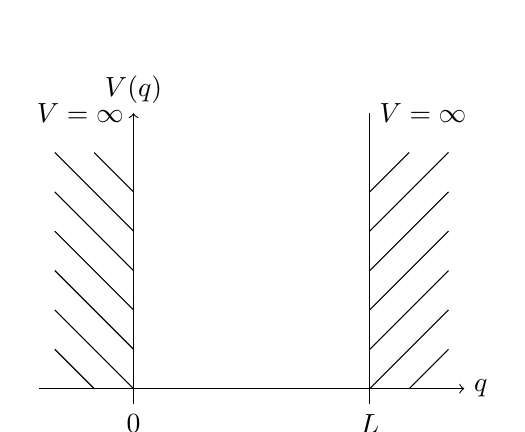
\begin{tikzpicture}
  \draw[->] (-1.2,0) -- (4.2,0) node[right] {$q$};
  \draw[->] (0,-0.2) -- (0,3.5) node[left]{$V=\infty$} node[above] {$V(q)$};
  \draw (0,0) +(0,0.2) -- +(0,-0.2) node[below] {$0$};
  \draw (3,0) +(0,0.2) -- +(0,-0.2) node[below] {$L$};
  \draw (3,0) -- (3,3.5) node[right]{$V=\infty$};
  \foreach \y in {0,0.5,...,2}
    \draw (3,\y) -- +(1,1) (0,\y) -- +(-1,1);
  \draw (3.5,0) -- (4,0.5);
  \draw (-0.5,0) -- (-1,0.5);
  \draw (3,2.5) -- (3.5,3);
  \draw (0,2.5) -- (-0.5,3);
\end{tikzpicture} 
\par\end{center}

The normalized eigenstates are:
\begin{align*}
\psi_{n}\left(q\right) & =\sqrt{\frac{2}{L}}\sin\left(\frac{n\pi}{L}q\right)\\
e_{n} & =n^{2}e_{0}
\end{align*}



\section{Square well}

\noindent \begin{center}
\begin{tikzpicture}
  \draw[->] (-4.7,0) -- (4.7,0) node[right] {$q$};
  \draw[->] (0,-0.2) -- (0,3.5) node[above] {$V(q)$};
  \draw (0,0) +(0,0.2) -- +(0,-0.2) node[below] {$0$};
  \draw (3,0) +(0,0.2) -- +(0,-0.2) node[below] {$\frac{L}{2}$};
  \draw (-3,0) +(0,0.2) -- +(0,-0.2) node[below] {$-\frac{L}{2}$};
  \draw (0,2) + (0.2,0) -- +(-0.2,0) node[left] {$V_0$};
  \draw (3,0) -- (3,2)
        (-3,0) -- (-3,2)
        (-4.7,2) -- (-3,2)
        (3,2) -- (4.7,2);
  \path (-4,1)node{I} (0.5,1) node{II} (4,1) node{III};
\end{tikzpicture} 
\par\end{center}

\begin{iiilist}

\iii Energy $E<V_{0}$ smaller than potential wall, leads to a bound
state.

Write the equation:
\begin{align*}
\left(-\frac{\hbar^{2}}{2m}\partial_{q}^{2}+V\left(q\right)\right)\psi\left(q\right) & =E\psi\left(q\right)\\
\partial_{q}^{2}\psi\left(q\right) & =-k\left(E\right)^{2}\psi\left(q\right)\\
k\left(E\right) & =+\sqrt{\frac{2m}{\hbar^{2}}\left(E-V\left(q\right)\right)}
\end{align*}
In the three regions I, II and III one gets:
\begin{align*}
k_{\text{I}}\left(E\right) & =\ii\abs{k_{\text{I}}\left(E\right)}\\
k_{\text{II}}\left(E\right) & =\abs{k_{\text{II}}\left(E\right)}\\
k_{\text{III}}\left(E\right) & =\ii\abs{k_{\text{III}}\left(E\right)}
\end{align*}
\iii Write the general solution:
\begin{align*}
\psi_{\text{I}\left(q\right)} & =A_{\text{I}}e^{\abs{k_{\text{I}}\left(E\right)}q}+B_{\text{I}}e^{-\abs{k_{\text{I}}\left(E\right)}q}\\
\psi_{\text{II}\left(q\right)} & =A_{\text{II}}e^{\ii\abs{k_{\text{II}}\left(E\right)}q}+B_{\text{II}}e^{-\ii\abs{k_{\text{II}}\left(E\right)}q}\\
\psi_{\text{III}\left(q\right)} & =A_{\text{III}}e^{\abs{k_{\text{I}}\left(E\right)}q}+B_{\text{III}}e^{-\abs{k_{\text{II}}\left(E\right)}q}
\end{align*}
\iii Normalization: $B_{\text{I}}=A_{\text{III}}=0$

Continuity: For a finite potential $\psi$ and $\partial_{q}\psi'$
are continuous.
\begin{align*}
\psi_{\text{I}}\left(-\frac{L}{2}\right) & =\psi_{\text{II}}\left(-\frac{L}{2}\right) & \partial_{q}\psi_{\text{I}}\left(-\frac{L}{2}\right) & =\partial_{q}\psi_{\text{II}}\left(-\frac{L}{2}\right)\\
\psi_{\text{II}}\left(\frac{L}{2}\right) & =\psi_{\text{III}}\left(\frac{L}{2}\right) & \partial_{q}\psi_{\text{II}}\left(\frac{L}{2}\right) & =\partial_{q}\psi_{\text{III}}\left(\frac{L}{2}\right)
\end{align*}
Now we have four equations and four variables, but one expects infinitely
many solutions.
\begin{align*}
\mathbb{M}\left(\begin{array}{c}
A_{\text{I}}\\
A_{\text{II}}\\
B_{\text{II}}\\
B_{\text{III}}
\end{array}\right) & =0 & \det\mathbb{M}\left(E\right) & \stackrel{!}{=}0
\end{align*}


\end{iiilist}

%DATE: Di 8.5.12


\section{The harmonic oscillator (in one dimension)}

The potential is:
\begin{align*}
V\left(\hat{q}\right) & =\frac{m\omega_{0}^{2}}{2}\hat{q}^{2}
\end{align*}
For all energies $e_{n}\in\mathbb{R}_{\ge0}$ we have:
\begin{align*}
\hat{H}\KET{e_{n}} & =e_{n}\KET{e_{n}}\\
\BraKet{e_{n}|e_{n}} & =1
\end{align*}
\begin{iiilist}

\iii The Schr�dinger equation is:
\begin{align*}
\left(\mins\frac{\hbar^{2}}{2m}\partial_{q}^{2}+\frac{m\omega_{0}^{2}}{2}q^{2}\right)\psi_{n}\left(q\right) & =e_{n}\psi_{n}\left(q\right) & \psi\left(q\to\pm\infty\right) & =0
\end{align*}
\iii Use dimensionless variables:
\begin{align*}
q & =\alpha x & \phi\left(x\right) & :=\psi_{n}\left(\alpha x\right)
\end{align*}
\begin{align*}
\left(\mins\frac{\hbar^{2}}{2m}\frac{1}{\alpha^{2}}\partial_{q}^{2}+\frac{m\omega_{0}^{2}}{2}\alpha^{2}q^{2}\right)\phi\left(q\right) & =e_{n}\phi\left(x\right)\\
\left(\partial_{x}^{2}-\frac{m^{2}\omega_{0}^{2}}{\hbar^{2}}\alpha^{4}x^{2}\right)\phi\left(q\right) & =\mins\frac{2m}{\hbar^{2}}\alpha^{2}e_{n}\phi\left(x\right)
\end{align*}
Choose:
\begin{align*}
\alpha & :=\sqrt{\frac{\hbar}{m\omega_{0}}} & \lambda & :=\frac{2e_{n}}{\hbar\omega_{0}}
\end{align*}
Then the problem reduces to:
\begin{align*}
\fbox{\ensuremath{\left(\partial_{x}^{2}+\left(\lambda-x^{2}\right)\right)\phi\left(x\right)=0\qquad\qquad}\ensuremath{\psi\left(x\to\pm\infty\right)}=0}
\end{align*}


\iii Check the asymptotic behavior, that is, when $x$ goes to $\pm\infty$:
\begin{align*}
\phi\left(x\right) & \approx\exp\left(\mins\frac{1}{2}x^{2}\right)
\end{align*}
Assume a solution:
\begin{align*}
\phi\left(x\right) & =u\left(x\right)\exp\left(\mins\frac{1}{2}x^{2}\right)
\end{align*}


\iii Then we get for $u\left(x\right)$ the differential equation:
\begin{align*}
\left(\partial_{x}^{2}-2x\partial_{x}+\left(\lambda-1\right)\right)u\left(x\right) & =0
\end{align*}
Solve this with a power series, by assuming, that $u\left(x\right)$
is analytic:
\begin{align*}
u\left(x\right) & =\sum_{n=0}^{\infty}a_{n}x^{n}
\end{align*}
This leads to the \quotedblbase{}recursion relation\textquotedblleft{}:
\begin{align*}
a_{n+2} & =\frac{\left(2n+1-\lambda\right)}{\left(n+1\right)\left(n+2\right)}a_{n}
\end{align*}
Or equivalently:
\begin{align*}
a_{n-2} & =\frac{\left(n-1\right)n}{\left(2n-3-\lambda\right)}a_{n}
\end{align*}


\iii Check again the asymptotic behavior, to get an idea, how $u\left(x\right)$
looks like, when $n\to\infty$:
\begin{align*}
\frac{a_{n+2}}{a_{n}} & \xrightarrow{n\gg1}\frac{2}{n}
\end{align*}
But we have
\begin{align*}
\exp\left(\mins\frac{x^{2}}{2}\right) & =\sum_{n=0}^{\infty}\underbrace{\frac{1}{n!}\left(\mins\frac{1}{2}\right)^{n}}_{=:c_{n}}x^{2n}=\sum_{n=0}^{\infty}c_{n}x^{2n}
\end{align*}
with:
\begin{align*}
\frac{c_{n+1}}{c_{n}}=\frac{n!}{\left(n+1\right)!}\cdot\left(\mins\frac{1}{2}\right)^{n+1}\cdot\left(\mins2\right)^{n}=\frac{\mins1}{2\left(n+1\right)} & \xrightarrow{n\gg1}\mins\frac{1}{2n}
\end{align*}
Therefore $u\left(x\to\infty\right)$ grows \noun{faster than} $\exp\left(\frac{1}{2}x^{2}\right)$
and therefore:
\begin{align*}
\exp\left(\mins\frac{1}{2}x^{2}\right)u\left(x\right) & \to\infty
\end{align*}
If the series does not stop, $\phi\left(x\right)$ is \emph{not} normalizable.

So there has to exist a \quotedblbase{}$n^{*}$\textquotedblleft{}
such that:
\begin{align*}
2n^{*}+1-\lambda & =0\\
\lambda & =2n^{*}+1\\
e_{n} & =\hbar\omega_{0}\left(n^{*}+\frac{1}{2}\right)
\end{align*}
This gives:
\begin{align*}
\psi_{n}\left(q\right) & =N_{n}\exp\left(\mins\frac{1}{2}\left(\frac{q}{\alpha}\right)^{2}\right)H_{n}\left(\frac{q}{\alpha}\right)
\end{align*}
The polynomials $H_{n}\left(x\right)$ are called the \noun{Hermite
polynomials} and are explicitly:
\begin{align*}
H_{n}\left(x\right) & =\left(-1\right)^{n}\sum_{k_{1}+2k_{2}=n}\frac{n!}{k_{1}!\cdot k_{2}!}\left(-1\right)^{k_{1}+k_{2}}\left(2x\right)^{k_{1}}
\end{align*}


$N_{n}$ is fixed by:
\begin{align*}
\int_{-\infty}^{\infty}\abs{\psi_{n}\left(q\right)}^{2}\dd q & =1
\end{align*}


\end{iiilist}

This looks like:

\noindent \begin{center}
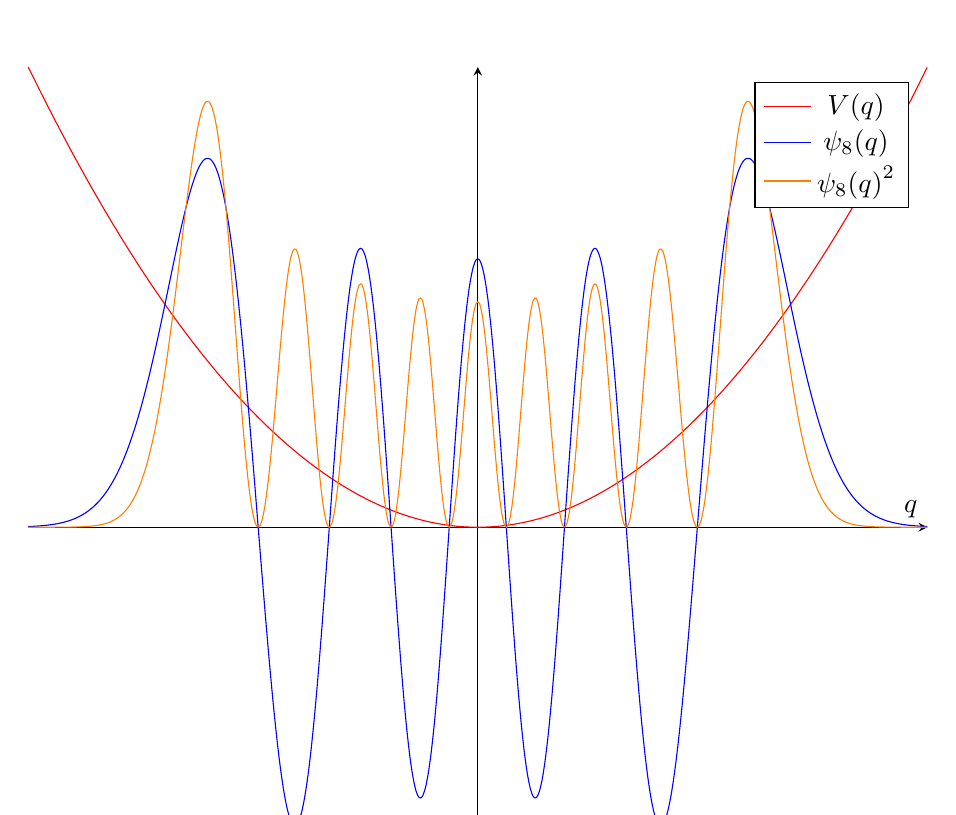
\begin{tikzpicture}
 \begin{axis}[width=13cm, axis x line=middle, axis y line=middle, xtick={0}, ytick={0}, xlabel=$q$,domain=-6:6,samples=300,smooth]
%  \addplot[green,mark=none] {(8*x^3-12*x)*exp(-x^2/2)*0.5};
%  \addlegendentry{$\psi_3 (q)$}
  \addplot[red,mark=none] {x^2*0.08};
  \addlegendentry{$V(q)$}
  \addplot[blue,mark=none] {(0.256*x^8-3.584*x^6+13.440*x^4-13.440*x^2+1.680)*exp(-x^2/2)};
  \addlegendentry{$\psi_8 (q)$}
\addplot[orange,mark=none] {((0.256*x^8-3.584*x^6+13.440*x^4-13.440*x^2+1.680)*exp(-x^2/2))^2*0.5};
  \addlegendentry{$\abs{\psi_8 (q)}^2$}
 \end{axis}
\end{tikzpicture} 
\par\end{center}

Then came Dirac:


\subsection{The number representation}

Introduce two operators:
\begin{align*}
 & \text{\quotedblbase destruction\textquotedblleft} &  & \text{\quotedblbase creation\textquotedblleft}\\
\hat{a} & =\sqrt{\frac{m\omega_{0}}{2\hbar}}\left(\hat{q}+\frac{\ii}{m\omega_{0}}\hat{p}\right) & \hat{a}^{\dagger} & =\sqrt{\frac{m\omega_{0}}{2\hbar}}\left(\hat{q}-\frac{\ii}{m\omega_{0}}\hat{p}\right)
\end{align*}
It is easy to calculate:
\begin{align*}
\left[\hat{a},\hat{a}^{\dagger}\right] & =1
\end{align*}
Introduce the \quotedblbase{}number\textquotedblleft{} operator:
\begin{align*}
\hat{n} & :=\hat{a}^{\dagger}\hat{a}
\end{align*}
Then we can find easily:
\begin{align*}
\hat{H} & =\frac{1}{2m}\hat{p}^{2}+\frac{m\omega_{0}^{2}}{2}\hat{q}^{2}=\hbar\omega_{0}\left(\hat{n}+\frac{1}{2}\right)
\end{align*}
Therefore the eigenstates of $\hat{n}$ are automatically the eigenstates
of $\hat{H}$.

It also satisfies:
\begin{align*}
\left[\hat{n},\hat{a}\right] & =\mins\hat{a} & \left[\hat{n},\hat{a}^{\dagger}\right] & =\hat{a}^{\dagger}
\end{align*}
We want to find $\KET{\sigma}$ such that:
\begin{align*}
\hat{n}\KET{\sigma} & =\sigma\KET{\sigma}
\end{align*}
We note:
\begin{align*}
\hat{n}\left(\hat{a}\KET{\sigma}\right) & =\left(\hat{n}\hat{a}\right)\KET{\sigma}=\left(\hat{a}\hat{n}-\left[\hat{a},\hat{n}\right]\right)\KET{\sigma}=\left(\hat{a}\hat{n}-\hat{a}\right)\KET{\sigma}=\left(\sigma-1\right)\KET{\sigma}
\end{align*}
$\hat{a}\KET{\sigma}$ is an eigenstate of $\hat{n}$ with eigenvalue
$\sigma-1$, so we get:
\begin{align*}
\hat{a}\KET{\sigma} & =N_{\sigma}\KET{\sigma-1}
\end{align*}
From $\BraKet{\sigma|\sigma}=\BraKet{\sigma-1|\sigma-1}=1$ follows:
\begin{align*}
\fbox{\ensuremath{\hat{a}\KET{\sigma}=\sqrt{\sigma}\KET{\sigma-1}}}
\end{align*}
Analogously we have:
\begin{align*}
\fbox{\ensuremath{\hat{a}^{\dagger}\KET{\sigma}=\sqrt{\sigma+1}\KET{\sigma+1}}}
\end{align*}
Take a $\sigma>0$ and apply $\hat{a}$ to $\KET{\sigma}$ many times
to get, that $\sigma$ must be an integer, because otherwise the normalization
constant $\sqrt{\sigma}$ would be imaginary.

There is a special state $\KET 0$, the \quotedblbase{}vacuum\textquotedblleft{}.

Let us call the states $\KET n$ for $n\in\mathbb{N}_{0}$.
\begin{align*}
\hat{n}\KET n & =n\KET n & \hat{a}\KET n & =\sqrt{n}\KET{n-1} & \hat{a}^{\dagger}\KET n & =\sqrt{n+1}\KET{n+1}
\end{align*}
\begin{align*}
\hat{H}\KET n & =e_{n}\KET n & e_{n} & =\hbar\omega_{0}\left(n+\frac{1}{2}\right)
\end{align*}
If we know $\KET 0$, we can construct an arbitrary $\KET n$:
\begin{align*}
\KET n & =\frac{1}{\sqrt{n!}}\left(\hat{a}^{\dagger}\right)^{n}\KET 0
\end{align*}
To calculate $\BraKet{q|0}$ we use $\hat{a}\KET 0=0$ and represent.
\begin{align*}
\BraKet{q|\hat{a}|0} & =0\\
\BraKet{q|\hat{q}+\frac{\ii}{m\omega_{0}}\hat{p}|0} & =0\\
\left(q+\frac{\ii}{m\omega_{0}}\left(\mins\ii\hbar\partial_{q}\right)\right)\psi_{0}\left(q\right) & =0\\
\left(\frac{\hbar}{m\omega_{0}}\partial_{q}+q\right)\psi_{0}\left(q\right) & =0\\
\psi_{0}\left(q\right) & =N_{0}\exp\left(\mins\frac{1}{2}\left(\frac{q}{\alpha}\right)^{2}\right)
\end{align*}
$N_{0}$ is fixed by normalization:
\begin{align*}
\int_{-\infty}^{\infty}\abs{\psi_{0}\left(q\right)}^{2}\dd q & =1
\end{align*}
For example $\psi_{1}\left(q\right)$ is given by:
\begin{align*}
\psi_{1}\left(q\right) & =\BraKet{q|1}=\BraKet{q|\hat{a}^{\dagger}|0}=\sqrt{\frac{m\omega_{0}}{2\hbar}}\left(q-\frac{\ii}{m\omega_{0}}\left(-\ii\hbar\partial_{q}\right)\right)\psi_{0}\left(q\right)=\\
 & =N_{0}\sqrt{\frac{m\omega_{0}}{2\hbar}}\left(q-\frac{\hbar}{m\omega_{0}}\partial_{q}\right)\exp\left(\mins\frac{1}{2}\left(\frac{q}{\alpha}\right)^{2}\right)=\\
 & =N_{1}\exp\left(\mins\frac{1}{2}\left(\frac{q}{\alpha}\right)^{2}\right)\cdot H_{1}\left(\frac{q}{\alpha}\right)
\end{align*}


%DATE: Do 10.5.12


\subsection{The dynamics of the harmonic oscillator}

The Hamiltonian is:
\begin{align*}
\hat{H} & =\frac{1}{2m}\hat{p}^{2}+\frac{m\omega_{0}^{2}}{2}\hat{q}^{2}
\end{align*}


In principal we need:
\begin{align*}
\hat{U}\left(t\right) & :=\exp\left(\mins\frac{\ii}{\hbar}\hat{H}t\right)=\exp\left(\mins\frac{\ii}{\hbar}\left(\frac{1}{2m}\hat{p}^{2}+\frac{m\omega_{0}^{2}}{2}\hat{q}^{2}\right)t\right)
\end{align*}
Let's calculate in the position representation:
\begin{align*}
\BraKet{q|\hat{U}\left(t\right)|q'} & =:U\left(q,q',t\right)
\end{align*}
Remember, what $\hat{U}$ does:
\begin{align*}
\KET{\psi\left(t\right)} & =\hat{U}\left(t\right)\KET{\psi\left(0\right)}
\end{align*}
In position representation this is:
\begin{align*}
\psi\left(q,t\right) & =\int U\left(q,q',t\right)\psi\left(q',0\right)\dd q'
\end{align*}
In some books the notation for $U\left(q,q',t\right)$ is $K\left(q,q',t\right)$.

\begin{align*}
U\left(q,q',t\right) & =\sum_{n}\exp\left(\mins\frac{\ii}{\hbar}e_{n}t\right)\BraKet{q|n}\BraKet{n|q'}=\\
 & =\sum_{n}\exp\left(\mins\ii\omega_{0}\left(n+\frac{1}{2}\right)t\right)N_{n}\exp\left(\mins\frac{1}{2}\left(\frac{q}{\alpha}\right)^{2}\right)H_{n}\left(\frac{q}{\alpha}\right)\cdot\\
 & \qquad\qquad\cdot\left(N_{n}\exp\left(-\frac{1}{2}\left(\frac{q'}{\alpha}\right)^{2}\right)H_{n}\left(\frac{q'}{\alpha}\right)\right)^{*}=\\
 & =\sum_{n}\exp\left(\mins\ii\omega_{0}\left(n+\frac{1}{2}\right)t\right)N_{n}^{2}\exp\left(\mins\frac{q^{2}+q'{}^{2}}{2\alpha^{2}}\right)H_{n}\left(\frac{q}{\alpha}\right)H_{n}\left(\frac{q'}{\alpha}\right)=\\
 & =\sqrt{\frac{m\omega_{0}}{2\pi\ii\hbar\sin\left(\omega_{0}t\right)}}\cdot\exp\left(\frac{\ii}{\hbar}\left(\frac{m\omega_{0}}{2\sin\left(\omega_{0}t\right)}\right)\left(q^{2}+q'{}^{2}\right)\cos\left(\omega_{0}t\right)-2qq'\right)
\end{align*}
To check this, consider the limes $\omega_{0}\to0$, for which we
get the free particle:
\begin{align*}
U\left(q,q',t\right) & \xrightarrow{\omega_{0}\to0}\sqrt{\frac{m}{2\pi\ii\hbar t}}\cdot\exp\left(\frac{\ii}{\hbar}\frac{m}{2t}\left(q-q'\right)^{2}\right)
\end{align*}
Let's try the Heisenberg picture:
\begin{align*}
\frac{\dd}{\dd t}\hat{q}_{H}\left(t\right) & =\frac{\ii}{\hbar}\left[H\left(\hat{q}_{H},\hat{p}_{H}\right),\hat{q}_{H}\right]=\frac{1}{m}\hat{p}_{H}\\
\frac{\dd}{\dd t}\hat{p}_{H}\left(t\right) & =\frac{\ii}{\hbar}\left[H\left(\hat{q}_{H},\hat{p}_{H}\right),\hat{p}_{H}\right]=-m\omega_{0}\hat{q}_{H}
\end{align*}
The initial conditions are:
\begin{align*}
\hat{q}_{H}\left(t=0\right) & =\hat{q}\\
\hat{p}_{H}\left(t=0\right) & =\hat{p}
\end{align*}


Remember the definition of an operator in the Heisenberg picture:
\begin{align*}
\hat{q}_{H} & =\exp\left(\frac{\ii}{\hbar}\hat{H}t\right)\hat{q}\exp\left(\mins\frac{\ii}{\hbar}\hat{H}t\right)
\end{align*}


Now we define the \noun{nested commutator} as
\begin{align*}
\left[\hat{B},\hat{A}\right]^{\left(0\right)} & :=\hat{A}\\
\left[\hat{B},\hat{A}\right]^{\left(n+1\right)} & :=\left[\hat{B},\left[\hat{B},\hat{A}\right]^{\left(n\right)}\right]
\end{align*}
and use the operator identity for $\lambda\in\mathbb{C}$ and arbitrary
operators $\hat{A},\hat{B}$:
\begin{align*}
\exp\left(\ii\lambda\hat{B}\right)\hat{A}\exp\left(\mins\ii\lambda\hat{B}\right) & =\sum_{n=0}^{\infty}\frac{\left(\ii\lambda\right)^{n}}{n!}\left[\hat{B},\hat{A}\right]^{\left(n\right)}\\
 & \approx\hat{A}+\ii\lambda\left[\hat{B},\hat{A}\right]+\frac{\left(\ii\lambda\right)^{2}}{2!}\left[\hat{B},\left[\hat{B},\hat{A}\right]\right]
\end{align*}
If $\left[\hat{A},\hat{B}\right]=0$, we get just $\hat{A}$.

If $\left[\hat{A},\left[\hat{A},\hat{B}\right]\right]=\left[\hat{B},\left[\hat{A},\hat{B}\right]\right]=0$,
we get $\hat{A}+\ii\lambda\left[\hat{B},\hat{A}\right]$.

Now we come back to the problem at hand:
\begin{align*}
\lambda & =\frac{t}{\hbar} & \hat{B} & =\hat{H} & \hat{A} & =\hat{q}
\end{align*}
We know:
\begin{align*}
\left[\hat{H},\hat{q}\right] & =\frac{1}{2m}\left[\hat{p}^{2},\hat{q}\right]+\underbrace{\left[V\left(\hat{q}\right),\hat{q}\right]}_{=0}=\frac{1}{2m}\left(\hat{p}\left[\hat{p},\hat{q}\right]+\left[\hat{p},\hat{q}\right]\hat{p}\right)=\mins\frac{\ii\hbar}{m}\hat{p}\\
\left[\hat{H},\hat{p}\right] & =\underbrace{\frac{1}{2m}\left[\hat{p}^{2},\hat{p}\right]}_{=0}+\frac{m\omega_{0}^{2}}{2}\left[\hat{q}^{2},\hat{p}\right]=\ii\hbar m\omega_{0}^{2}\hat{q}
\end{align*}
Together this inductively gives:
\begin{align*}
\hat{q}_{H}\left(t\right) & =\hat{q}\cos\left(\omega_{0}t\right)+\frac{1}{m\omega_{0}}\hat{p}\sin\left(\omega_{0}t\right)\\
\hat{p}_{H}\left(t\right) & =m\omega_{0}\hat{q}\sin\left(\omega_{0}t\right)+\hat{p}\cos\left(\omega_{0}t\right)
\end{align*}



\section{The tunneling effect}

Look at the potential:

\noindent \begin{center}
\begin{tikzpicture}
  \draw[->] (-5.2,0) -- (5.2,0) node[right] {$q$};
  \draw[->] (0,-0.2) -- (0,3.5) node[above] {$V(q)$};
  \draw (0,0) +(0,0.2) -- +(0,-0.2) node[below] {$0$};
  \draw (2,0) +(0,0.2) -- +(0,-0.2) node[below] {$\frac{d}{2}$};
  \draw (-2,0) +(0,0.2) -- +(0,-0.2) node[below] {$-\frac{d}{2}$};
  \draw (0,2) + (0.2,0) -- +(-0.2,0) node[above left] {$V_0$};
  \draw (2,0) -- (2,2) -- (-2,2) -- (-2,0);
  \path (-2.5,1)node{I} (0.5,1) node{II} (2.5,1) node{III};
  %Wellenpfeile
  \draw[->] (-5,1.5) -- node[above]{$A_\text{I} e^{\ii kq}$} (-3,1.5);
  \draw[->] (-3,0.5) -- node[above]{$R e^{\mins \ii kq}$} (-5,0.5);
  \draw[->] (3,1) -- node[above]{$T e^{ \ii kq}$} (5,1);
\end{tikzpicture} 
\par\end{center}

The problem is unbounded and therefore the spectrum is continuous
and every energy $E\in\mathbb{R}_{>0}$ is allowed.

Imagine that we inject the particle from the left with a certain energy
$E$.
\begin{align*}
k & :=\frac{\sqrt{2mE}}{\hbar} & k_{V} & :=\frac{\sqrt{2m\left(V_{0}-E\right)}}{\hbar}
\end{align*}
The goal is to find $R$ and $T$ as functions of the Energy $E$,
the height $V_{0}$ and width $d$ of the potential.

Business as usual:

The boundary condition is, that $A_{\text{I}}$ is know and the coefficient
of $e^{\mins\ii kq}$ in the region III is zero. We consider only
$E<V_{0}$.
\begin{align*}
\psi_{\text{I}}\left(q\right) & =A_{\text{I}}e^{\ii kq}+Re^{-\ii kq}\\
\psi_{\text{II}}\left(q\right) & =A_{\text{II}}e^{k_{V}q}+B_{\text{II}}e^{-k_{V}q}\\
\psi_{\text{III}}\left(q\right) & =Te^{\ii kq}
\end{align*}
We have the four variables $R,T,A_{\text{II}}$ and $B_{\text{II}}$.
Know we impose the matching conditions:
\begin{align*}
\psi_{\text{I}}\left(\mins\frac{d}{2}\right) & =\psi_{\text{II}}\left(\mins\frac{d}{2}\right) & \psi_{\text{I}}'\left(\mins\frac{d}{2}\right) & =\psi_{\text{II}}'\left(\mins\frac{d}{2}\right)\\
\psi_{\text{I}}\left(\frac{d}{2}\right) & =\psi_{\text{II}}\left(\frac{d}{2}\right) & \psi_{\text{I}}'\left(\frac{d}{2}\right) & =\psi_{\text{II}}'\left(\frac{d}{2}\right)
\end{align*}
This system looks like:
\begin{align*}
\mathbb{M}\cdot\left(\begin{array}{c}
B\\
A_{\text{II}}\\
B_{\text{II}}\\
T
\end{array}\right) & =A_{\text{I}}\left(\begin{array}{c}
\mins e^{\mins\ii k\frac{d}{2}}\\
\mins\ii ke^{\ii k\frac{d}{2}}\\
0\\
0
\end{array}\right)
\end{align*}
For $k_{V}d\gg1$ this roughly gives:
\begin{align*}
T\left(E\right) & \sim A_{\text{I}}e^{\mins\frac{k_{V}\left(E\right)d}{2}}\\
\frac{T\left(E,d\right)}{T\left(E,d'\right)} & \sim e^{\mins\frac{k_{V}\left(E\right)}{2}\left(d-d'\right)}
\end{align*}



\section{Two formal consequences of the position representation of the Schr�dinger
equation}


\subsection{Oscillation theorem \textmd{(1D, bounded)}}

If $\BraKet{q|e_{n}}$ has $k$-nodes, that means $\psi_{n}\left(q\right)=0$
is $k$ times, then $\BraKet{q|e_{n+1}}$ has $k+1$ nodes.

\noindent \begin{center}
\begin{tikzpicture}
 \begin{axis}[width=10cm, axis x line=middle, axis y line=middle, xtick={0}, ytick={0}, xlabel=$q$,domain=-6:6,samples=150,smooth]
  \addplot[mark=none] {sin(x*114.6)*exp(-x^2*0.1)};
  \addplot[mark=*] coordinates {(-4.71,0) (-3.14,0) (-1.57,0) (0,0) (1.57,0) (3.14,0) (4.71,0)};
 \end{axis}
\end{tikzpicture} 
\par\end{center}


\subsection{The continuity equation}

Let $\psi\left(\vec{q},t\right)$ solve the Schr�dinger equation for
the Hamilton operator $\hat{H}=\frac{\hat{\vec{p}}^{2}}{2m}+V\left(\hat{\vec{q}}\right)$.
Since $\hat{H}$ is Hermitian, $V\left(\vec{q}\right)$ has to be
real and solve:
\begin{align*}
\ii\hbar\partial_{t}\psi\left(\vec{q},t\right) & =\left(-\frac{\hbar^{2}}{2m}\nabla^{2}+V\left(\vec{q}\right)\right)\psi\left(\vec{q},t\right)\\
-\ii\hbar\partial_{t}\psi^{*}\left(\vec{q},t\right) & =\left(-\frac{\hbar^{2}}{2m}\nabla^{2}+V\left(\vec{q}\right)\right)\psi^{*}\left(\vec{q},t\right)
\end{align*}
This gives:
\begin{align*}
\partial_{t}\abs{\psi}^{2} & =\partial_{t}\left(\psi\psi^{*}\right)=\left(\partial_{t}\psi\right)\psi^{*}+\psi\left(\partial_{t}\psi^{*}\right)=\\
 & =\psi^{*}\left(\frac{1}{\ii\hbar}\left(-\frac{\hbar^{2}}{2m}\nabla^{2}+V\left(\vec{q}\right)\right)\psi\right)+\psi\left(\frac{-1}{\ii\hbar}\left(-\frac{\hbar^{2}}{2m}\nabla^{2}+V\left(\vec{q}\right)\right)\psi^{*}\right)=\\
 & =\psi^{*}\left(-\frac{\hbar}{2m\ii}\nabla^{2}\psi\right)+\psi\left(\frac{\hbar}{2m\ii}\nabla^{2}\psi^{*}\right)=\\
 & =\frac{\hbar}{2m\ii}\left(\psi\nabla^{2}\psi^{*}-\psi^{*}\nabla^{2}\psi\right)=\\
 & =\frac{\hbar}{2m\ii}\nabla\left(\psi\nabla\psi^{*}-\psi^{*}\nabla\psi\right)
\end{align*}
Therefore we have the continuity equation:
\begin{align*}
\partial_{t}\abs{\psi}^{2}-\frac{\hbar}{2m\ii}\nabla\left(\psi\nabla\psi^{*}-\psi^{*}\nabla\psi\right) & =0
\end{align*}


Define the probability density $\varrho_{\psi}\left(\vec{q},t\right):=\abs{\psi\left(\vec{q},t\right)}^{2}$
and the probability current:
\begin{align*}
\vec{j}_{\psi}\left(\vec{q},t\right) & :=-\frac{\ii\hbar}{2m}\left(\psi^{*}\nabla\psi-\psi\nabla\psi^{*}\right)
\end{align*}
They are related by 
\begin{align*}
\partial_{t}\varrho_{\psi}\left(\vec{q},t\right)+\nabla\vec{j}_{\psi}\left(\vec{q},t\right) & =0
\end{align*}
and we can interpret them as expectation values:
\begin{align*}
\varrho_{\psi}\left(\vec{q},t\right) & =\abs{\psi\left(\vec{q},t\right)}^{2}=\abs{\left\langle \hat{\vec{q}}|\psi\left(t\right)\right\rangle }^{2}=\BRA{\hat{\vec{q}}}\underbrace{\KET{\psi\left(t\right)}\BRA{\psi\left(t\right)}}_{=:\hat{\varrho}}\KET{\hat{\vec{q}}}=\BraKet{\hat{\vec{q}}|\hat{\varrho}|\hat{\vec{q}}}
\end{align*}
\begin{align*}
\vec{j}\left(\vec{q},t\right) & =\frac{-\ii\hbar}{2m}\left(\psi^{*}\nabla\psi-\psi\nabla\psi^{*}\right)=\frac{-\ii\hbar}{2m}\left(\left\langle \psi|\vec{q}\right\rangle \nabla\left\langle \vec{q}|\psi\right\rangle -\left\langle \vec{q}|\psi\right\rangle \nabla\left\langle \psi|\vec{q}\right\rangle \right)=\\
 & =\frac{-1}{2m}\left(\left\langle \vec{q}|\hat{\vec{p}}|\psi\right\rangle \left\langle \psi|\vec{q}\right\rangle -\left\langle \vec{q}|\psi\right\rangle \left\langle \psi|\hat{\vec{p}}|\vec{q}\right\rangle \right)=\\
 & =\frac{-1}{2m}\BRA{\vec{q}}\underbrace{\left(\hat{\vec{p}}\KET{\psi}\BRA{\psi}-\KET{\psi}\BRA{\psi}\hat{\vec{p}}\right)}_{=\left[\hat{\vec{p}},\hat{\varrho}\right]}\KET{\vec{q}}=\frac{-1}{2m}\BRA{\vec{q}}\underbrace{\left[\hat{\vec{p}},\hat{\varrho}\right]}_{=:-2m\hat{\vec{j}}}\KET{\vec{q}}=\BraKet{\vec{q}|\hat{\vec{j}}|\vec{q}}
\end{align*}


%DATE: Di 15.5.12


\chapter{Symmetries, Rotations and Angular momentum}

Remember from classical mechanics:

A symmetry is a physical operation that leaves the system invariant.

In classical mechanics this means we change $\vec{q}$ and $\vec{p}$.

Examples:
\begin{itemize}
\item For $\mathcal{R}\in\text{SL}_{n}\left(\mathbb{R}\right)$, that means
$\mathcal{R}^{-1}=\mathcal{R}^{T}$ and $\det\left(\mathcal{R}\right)=1$,
we define:
\begin{align*}
\vec{q}' & =\mathcal{R}\vec{q}\\
\vec{p}' & =\mathcal{R}\vec{p}
\end{align*}
This leaves a Lagrangian of the Form ${\displaystyle \mathscr{L}\left(\vec{q},\dot{\vec{q}}\right)=\frac{m}{2}\abs{\dot{\vec{q}}}^{2}-V\left(\abs{\vec{q}}\right)}$.
$\Rightarrow$ $\left\{ H,\vec{L}\right\} =0$
\item The translation $\vec{q}'=\vec{q}+\vec{q}_{0}$ leaves the free particle
with Lagrangian
\begin{align*}
\mathscr{L}\left(\vec{q},\dot{\vec{q}},t\right) & =\frac{m}{2}\abs{\dot{\vec{q}}}^{2}
\end{align*}
invariant and therefore $\left\{ H,\vec{p}\right\} =0$.
\item Emmy Noether: Symmetry $\Rightarrow$ Existence of a constant of motion
\end{itemize}

\section{The tensor product in quantum mechanics}

Consider two degrees of freedom (for example two particles in one
dimension), described by states in $\mathcal{H}^{\left(1\right)},\mathcal{H}^{\left(2\right)}$.

A postulate of quantum mechanics says, that the composite system is
described by a state in the Hilbert space $\mathcal{H}=\mathcal{H}^{\left(1\right)}\otimes\mathcal{H}^{\left(2\right)}$.
This space is called \noun{tensor product}.

So the dimension is $\dim\mathcal{H}=\dim\left(\mathcal{H}^{\left(1\right)}\right)\cdot\dim\left(\mathcal{H}^{\left(2\right)}\right)$.

If $\KET{\psi^{\left(1\right)}}\in\mathcal{H}^{\left(1\right)}$,
$\KET{\psi^{\left(2\right)}}\in\mathcal{H}^{\left(2\right)}$ then
$\KET{\psi^{\left(1\right)}}\otimes\KET{\psi^{\left(2\right)}}\in\mathcal{H}^{\left(1\right)}\otimes\mathcal{H}^{\left(2\right)}=\mathcal{H}$.

If $\hat{A}^{\left(1\right)}$ acts on $\mathcal{H}^{\left(1\right)}$
and $\hat{A}^{\left(2\right)}$ acts on $\mathcal{H}^{\left(2\right)}$,
then $\hat{A}^{\left(1\right)}\otimes\hat{A}^{\left(2\right)}$ acts
on $\mathcal{H}$ as follows:
\begin{align*}
\left(\hat{A}^{\left(1\right)}\otimes\hat{A}^{\left(2\right)}\right)\left(\KET{\psi^{\left(1\right)}}\otimes\KET{\psi^{\left(2\right)}}\right) & =\left(\hat{A}^{\left(1\right)}\KET{\psi^{\left(1\right)}}\otimes\hat{A}^{\left(2\right)}\KET{\psi^{\left(2\right)}}\right)
\end{align*}
\begin{align*}
\hat{A}^{\left(1\right)} & \mapsto\hat{A}^{\left(1\right)}\otimes\hat{I}^{\left(2\right)}\\
\hat{A}^{\left(2\right)} & \mapsto\hat{I}^{\left(1\right)}\otimes\hat{A}^{\left(2\right)}\\
\left[\hat{A}^{\left(1\right)},\hat{A}^{\left(2\right)}\right] & =0
\end{align*}
For $\KET{\psi}=\KET{\psi^{\left(1\right)}}\otimes\KET{\psi^{\left(2\right)}}$
and $\KET{\varphi}=\KET{\varphi^{\left(1\right)}}\otimes\KET{\varphi^{\left(2\right)}}$
we have the scalar product:
\begin{align*}
\BraKet{\varphi|\psi} & =\BraKet{\varphi^{\left(1\right)}|\psi^{\left(1\right)}}\BraKet{\varphi^{\left(2\right)}|\psi^{\left(2\right)}}
\end{align*}


With all this together one can write any operator $\hat{A}$ and any
Ket $\KET{\psi}$:
\begin{align*}
\hat{A} & =\sum_{n.m}c_{n,m}\hat{A}_{n}^{\left(1\right)}\otimes\hat{A}_{m}^{\left(2\right)}\\
\KET{\psi} & =\sum_{n,m}a_{n,m}\KET{\psi_{n}^{\left(1\right)}}\otimes\KET{\psi_{m}^{\left(2\right)}}\stackrel{\text{i.A.}}{\not=}\KET{\varphi^{\left(1\right)}}\otimes\KET{\varphi^{\left(2\right)}}
\end{align*}
A state in the form $\KET{\psi^{\left(1\right)}}\otimes\KET{\psi^{\left(2\right)}}$
is called \emph{separable}.

If a state is not separable, it is called \emph{entangled}.

For example:
\begin{align*}
\left(\hat{A}^{\left(1\right)}\otimes\hat{I}^{\left(2\right)}+\hat{I}\otimes\hat{A}^{\left(2\right)}\right)^{2} & =\left(\hat{A}^{\left(1\right)}\right)^{2}\otimes\hat{I}^{\left(2\right)}+2\hat{A}^{\left(1\right)}\otimes\hat{A}^{\left(2\right)}+\hat{I}\otimes\left(\hat{A}^{\left(2\right)}\right)^{2}
\end{align*}
Now we can understand better:
\begin{align*}
\hat{q}_{\alpha}\KET{\vec{q}} & =q_{\alpha}\KET{\vec{q}}
\end{align*}
$\KET{\vec{q}}$ is just a compact way to write:
\begin{align*}
\KET{\vec{q}} & =\KET{q_{x},q_{y},q_{z}}:=\KET{q_{x}}\otimes\KET{q_{y}}\otimes\KET{q_{z}}
\end{align*}



\section{Rotations and angular momentum}

Come back to classical mechanics. We know, that $\vec{L}=\vec{q}\times\vec{p}$
\quotedblbase{}generates\textquotedblleft{} rotations $\mathcal{R}\left(\vec{n},\dd\vartheta\right)$
around an normalized axis $\vec{n}$ with the angle $\dd\vartheta$.
\begin{align*}
f\left(\vec{q},\vec{p}\right) & \to f\left(\vec{q}',\vec{p}'\right)=f\left(\mathcal{R}\left(\vec{n},\dd\vartheta\right)\vec{q},\mathcal{R}\left(\vec{n},\dd\vartheta\right)\vec{p}\right)\approx f\left(\vec{q},\vec{p}\right)+\dd\vartheta\left\{ \underbrace{\vec{L}\cdot\vec{n}}_{\text{Generator}},f\left(\vec{q},\vec{p}\right)\right\} +O\left(\left(\dd\vartheta\right)^{2}\right)
\end{align*}
Another example:
\begin{align*}
f\left(\vec{q}\left(t\right),\vec{p}\left(t\right)\right) & \to f\left(\vec{q}\left(t+\delta t\right),\vec{p}\left(t+\delta t\right)\right)\approx f\left(\vec{q},\vec{p}\right)+\dd t\left\{ H,f\left(\vec{q},\vec{p}\right)\right\} 
\end{align*}
Explicit calculation shows:
\begin{align*}
\left\{ L_{i},L_{j}\right\}  & =\varepsilon_{ijk}L_{k}
\end{align*}


In quantum mechanics we \noun{define} angular momentum $\vec{j}$
as the generator of rotations. Define:
\begin{align*}
\KET{\psi^{\mathcal{R}}} & =\hat{D}\left(\mathcal{R}\right)\KET{\psi}=e^{-\frac{\ii}{\hbar}\left(\vec{j}\cdot\vec{n}\right)\theta}\KET{\psi}
\end{align*}
Check out, how an operator $\hat{A}$ changes:
\begin{align*}
\hat{A}^{\mathcal{R}} & =\hat{D}\left(\mathcal{R}\right)^{\dagger}\hat{A}\hat{D}\left(\mathcal{R}\right)\xrightarrow{\theta\to\dd\theta}\hat{A}+\frac{\ii\dd\theta}{\hbar}\left[\vec{j}\cdot\vec{n},\hat{A}\right]+O\left(\dd\theta^{2}\right)
\end{align*}
We want, that the group properties of the $\mathcal{R}$'s, which
are
\begin{align*}
\mathcal{R}\left(\vec{n},0\right) & =E_{3}\\
\mathcal{R}\left(\vec{n}_{1},\theta_{1}\right)\mathcal{R}\left(\vec{n}_{2},\theta_{2}\right) & =\mathcal{R}\left(\vec{n}\left(\vec{n}_{1},\vec{n}_{2}\right),\theta\left(\theta_{1},\theta_{2}\right)\right)\quad\text{(cf. Goldstein Classical Mechanics)}\\
\mathcal{R}\left(\vec{n},\theta\right)^{-1} & =\mathcal{R}\left(\vec{n},-\theta\right)\\
\left(\mathcal{R}_{1}\mathcal{R}_{2}\right)\mathcal{R}_{3} & =\mathcal{R}_{1}\left(\mathcal{R}_{2}\mathcal{R}_{3}\right)
\end{align*}
go into the $\hat{D}$'s.
\begin{align*}
\hat{D}\left(\vec{n},0\right) & =\hat{I}\\
\hat{D}_{1}\left(\vec{n}_{1},\theta_{1}\right)\hat{D}_{2}\left(\vec{n}_{2},\theta_{2}\right) & =\hat{D}\left(\vec{n}\left(\vec{n}_{1},\vec{n}_{2}\right),\theta\left(\theta_{1},\theta_{2}\right)\right)\\
\hat{D}\left(\vec{n},\theta\right)^{-1} & =\hat{D}\left(\vec{n},-\theta\right)\\
\left(\hat{D}_{1}\hat{D}_{2}\right)\hat{D}_{3} & =\hat{D}_{1}\left(\hat{D}_{2}\hat{D}_{3}\right)
\end{align*}
In particular we want the $\hat{D}$'s version of:
\begin{align*}
\mathcal{R}\left(\vec{e}_{x},\varepsilon\right)\mathcal{R}\left(\vec{e}_{y},\varepsilon\right)-\mathcal{R}\left(\vec{e}_{y},\varepsilon\right)\mathcal{R}\left(\vec{e}_{x},\varepsilon\right) & \approx\left(\begin{array}{ccc}
1 & 0 & 0\\
0 & 1-\frac{\varepsilon^{2}}{2} & -\varepsilon\\
0 & \varepsilon & 1-\frac{\varepsilon^{2}}{2}
\end{array}\right)\left(\begin{array}{ccc}
1-\frac{\varepsilon^{2}}{2} & 0 & \varepsilon\\
0 & 1 & 0\\
-\varepsilon & 0 & 1-\frac{\varepsilon^{2}}{2}
\end{array}\right)-\\
 & \quad-\left(\begin{array}{ccc}
1-\frac{\varepsilon^{2}}{2} & 0 & \varepsilon\\
0 & 1 & 0\\
-\varepsilon & 0 & 1-\frac{\varepsilon^{2}}{2}
\end{array}\right)\left(\begin{array}{ccc}
1 & 0 & 0\\
0 & 1-\frac{\varepsilon^{2}}{2} & -\varepsilon\\
0 & \varepsilon & 1-\frac{\varepsilon^{2}}{2}
\end{array}\right)=\\
 & =\mathcal{R}\left(\vec{e}_{z},\varepsilon^{2}\right)-E_{3}=\left(\begin{array}{ccc}
0 & -\varepsilon^{2} & 0\\
\varepsilon^{2} & 0 & 0\\
0 & 0 & 0
\end{array}\right)
\end{align*}
So we want:
\begin{align*}
\left[\hat{D}\left(\vec{e}_{x},\varepsilon\right),\hat{D}\left(\vec{e}_{y},\varepsilon\right)\right] & =\hat{D}\left(\vec{e}_{z},\varepsilon^{2}\right)-\hat{I}+O\left(\varepsilon^{3}\right)
\end{align*}
Use
\begin{align*}
\hat{D}\left(\vec{e}_{i},\varepsilon\right) & =\exp\left(-\frac{\ii}{\hbar}\hat{J}_{i}\varepsilon\right)\approx1-\frac{\ii}{\hbar}\hat{J}_{i}\varepsilon+\left(-\frac{\ii}{\hbar}\right)^{2}\frac{1}{2}\hat{J}_{i}^{2}\varepsilon^{2}+\ldots
\end{align*}
to get:
\begin{align*}
\left[\hat{J}_{i},J_{j}\right] & =\ii\hbar\varepsilon_{ijk}\hat{J}_{k}
\end{align*}
Funny remark: Take the spin $\hat{\vec{s}}$ and calculate:
\begin{align*}
\exp\left(-\frac{\ii}{\hbar}\hat{s}_{z}\theta\right)\KET + & =\exp\left(-\ii\frac{\theta}{2}\right)\KET +
\end{align*}
For electrons you need a rotation of $4\pi$ to come back to the same
state.

%DATE: Di 22.5.12


\section{Eigenstates and eigenvalues of $\hat{\vec{j}}$}

First (again) notice, that since $\left[\hat{J}_{i},\hat{J}_{k}\right]\not=0$
for $i\not=k$ there is not any common eigenstate for the $\vec{J}$'s,
but we know:
\begin{align*}
\left[\abs{\hat{\vec{J}}}^{2},\hat{J}_{i}\right]:=\left[\hat{\vec{J}}^{2},\hat{J}_{i}\right] & =0
\end{align*}
Therefore we can find a basis $\KET{a,b}$ with:
\begin{align*}
\hat{J}^{2}\KET{a,b} & =a\KET{a,b}\\
\hat{J}_{z}\KET{a,b} & =b\KET{a,b}
\end{align*}
Now we introduce:
\begin{align*}
\hat{J}_{\pm} & :=\hat{J}_{x}\pm\ii\hat{J}_{y}\\
\hat{J}_{\pm}^{\dagger} & =\hat{J}_{\mp}
\end{align*}
Note that this gives:
\begin{align*}
\left[\hat{J}^{2},\hat{J}_{\pm}\right] & =0 & \left[\hat{J}_{+},\hat{J}_{-}\right] & =2\hbar\hat{J}_{z} & \left[\hat{J}_{z},\hat{J}_{\pm}\right] & =\pm\hbar\hat{J}_{\pm}
\end{align*}
The trick is always the same:
\begin{align*}
\hat{J}_{z}\left(\hat{J}_{\pm}\KET{a,b}\right) & =\hat{J}_{z}\hat{J}_{\pm}\KET{a,b}=\left(\hat{J}_{\pm}\hat{J}_{z}+\left[\hat{J_{z}},\hat{J}_{\pm}\right]\right)\KET{a,b}=\\
 & =\hat{J}_{\pm}b\KET{a,b}\pm\hbar\hat{J}_{\pm}\KET{a,b}=\left(b\pm\hbar\right)\hat{J}_{\pm}\KET{a,b}
\end{align*}
Therefore $\hat{J}_{\pm}\KET{a,b}$ is an eigenstate of $\hat{J}_{z}$
with the eigenvalue $b\pm\hbar$:
\begin{align*}
\hat{J}_{\pm}\KET{a,b} & =N^{\pm}\left(a,b\right)\KET{a,b\pm\hbar}
\end{align*}
Now we show, that $\abs b$ has an upper limit. Consider
\begin{align*}
\left\langle a,b|\hat{J}_{+}\hat{J}_{+}^{\dagger}|a,b\right\rangle +\left\langle a,b|\hat{J}_{+}^{\dagger}\hat{J}_{+}|a,b\right\rangle  & \in\mathbb{R}_{\ge0}
\end{align*}
and:
\begin{align*}
\hat{J}_{+}\hat{J}_{+}^{\dagger}+\hat{J}_{+}^{\dagger}\hat{J}_{+} & =\hat{J}_{+}\hat{J}_{-}+\hat{J}_{-}\hat{J}_{+}=2\left(\hat{J}^{2}-\hat{J}_{z}^{2}\right)
\end{align*}
Then we get:
\begin{align*}
0\le & \left\langle a,b|\hat{J}^{2}-\hat{J}_{z}^{2}|a,b\right\rangle =\left\langle a,b|a-b^{2}|a,b\right\rangle =a-b^{2}\\
a & \ge b^{2}\\
\abs b & \le\sqrt{a}
\end{align*}
This means, that there is a $b_{\text{max}}$ defined by:
\begin{align*}
\hat{J}_{+}\KET{a,b_{\text{max}}} & =0
\end{align*}
From this equation we get
\begin{align*}
\hat{J}_{-}\hat{J}_{+}\KET{a,b_{\text{max}}} & =0
\end{align*}
and:
\begin{align*}
\hat{J}^{2}-\hat{J}_{z}^{2}-\hbar\hat{J}_{z} & =a-b_{\text{max}}^{2}-\hbar b_{\text{max}}=0
\end{align*}
This finally leads to:
\begin{align*}
a & =b_{\text{max}}\left(b_{\text{max}}+\hbar\right)
\end{align*}
Analogously we get for $\hat{J}_{-}$:
\begin{align*}
\hat{J}_{-}\KET{a,b_{\text{min}}} & =0
\end{align*}
From this equation we get
\begin{align*}
\hat{J}_{+}\hat{J}_{-}\KET{a,b_{\text{min}}} & =0
\end{align*}
and:
\begin{align*}
\hat{J}^{2}-\hat{J}_{z}^{2}+\hbar\hat{J}_{z} & =a-b_{\text{min}}^{2}+\hbar b_{\text{min}}=0
\end{align*}
This finally leads to:
\begin{align*}
a & =b_{\text{min}}\left(b_{\text{min}}-\hbar\right)
\end{align*}
A solution is $b_{\text{max}}=-b_{\text{min}}$ and for a $n\in\mathbb{Z}$:
\begin{align*}
b_{\text{max}} & =b_{\text{min}}+n\hbar\\
b_{\text{max}}-b_{\text{mini}}=2b_{\text{max}} & =n\hbar\\
b_{\text{max}} & =\frac{n}{2}\hbar\\
a & =\frac{n}{2}\hbar\left(\frac{n}{2}\hbar+\hbar\right)=\hbar^{2}\underbrace{\frac{n}{2}}_{=:j}\left(\frac{n}{2}+1\right)
\end{align*}
Some names:

$j\in\frac{1}{2}\mathbb{Z}$ is called \emph{the total angular momentum
quantum number} and
\begin{align*}
m\in & \left\{ -j,\ldots,-j+1,\ldots,j-1,j\right\} 
\end{align*}
is called \emph{the magnetic quantum number}:
\begin{align*}
b & =m\hbar & a & =\hbar^{2}j\left(j+1\right)
\end{align*}
\begin{align*}
\hat{J}^{2}\KET{j,m} & =\hbar^{2}j\left(j+1\right)\KET{j,m}\\
\hat{J}_{z}\KET{j,m} & =\hbar m\KET{j,m}
\end{align*}
With a bit of algebra we get:
\begin{align*}
\hat{J}_{\pm}\KET{j,m} & =\hbar\sqrt{\left(j\mp m\right)\left(j\pm m+1\right)}\KET{j,m\pm1}
\end{align*}



\section{Irreducible representations of the rotation operators}

We want to construct the matrix representations of $\hat{D}\left(\vec{n},\theta\right)$.

In particular in the eigenbasis of $\hat{J}^{2}$ and $\hat{J}_{z}$.

Remember:
\begin{align*}
\hat{D}\left(\vec{n},\theta\right) & =e^{-\frac{\ii}{\hbar}\hat{\vec{J}}\cdot\vec{n}\theta}
\end{align*}
We want:
\begin{align*}
\left\langle j,m|\hat{D}\left(\vec{n},\theta\right)|j',m'\right\rangle  & =D_{jm}^{j'm'}\left(\vec{n},\theta\right)
\end{align*}
First note:, because $\left[\hat{\vec{J}}^{2},\hat{\vec{J}}\cdot\vec{n}\right]=0$.
\begin{align*}
D_{jm}^{j'm'}\left(\vec{n},\theta\right) & =D_{mm'}^{\left(j\right)}\left(\vec{n},\theta\right)\delta_{jj'}
\end{align*}
The physical reason is, that a rotation doesn't change magnitudes
like $j$.

${\displaystyle j=\frac{1}{2}}$ gives a $2\times2$-Matrix for $D$,
because the basis is $\KET{\frac{1}{2},-\frac{1}{2}}$ and $\KET{\frac{1}{2},\frac{1}{2}}$.

\noindent \begin{center}
$\left(\phantom{\begin{array}{c}a\\a\\a\\a\\a\\a\\a\\a\\a\\a\\a\end{array}}\right.$
\begin{tikzpicture}[baseline=(current bounding box.west)] 
  %j=1/2
  \node (j12) at (0,0) {$\Bigg( \quad j=\frac{1}{2} \quad \Bigg)$};
  \draw[<->] ($(j12.315) + (0.4,0) $) -- node[right]{2} ($ (j12.45) + (0.4,0) $);
  \draw[<->] ($(j12.45) + (0.3,0) $) -- node[above]{2} ($ (j12.135) + (-0.3,0) $);
  %j=1
  \node (j1) at (2.5,-2) {$\Bigg( \quad j=1 \quad \Bigg)$};
  \draw[<->] ($(j1.315) + (0.4,0) $) -- node[right]{3} ($ (j1.45) + (0.4,0) $);
  \draw[<->] ($(j1.45) + (0.3,0) $) -- node[above]{3} ($ (j1.135) + (-0.3,0) $);
  \node at (2.5,0) {0};
  \node at (0,-2) {0};
  \node at (4,-3) {$\ddots$};
\end{tikzpicture}
$\left.\phantom{\begin{array}{c}a\\a\\a\\a\\a\\a\\a\\a\\a\\a\\a\end{array}}\right)$
\par\end{center}

This is the matrix representation of a rotation operator $\hat{D}\left(\vec{n},\theta\right)$
in the basis $\KET{j,m}$ ordered as
\begin{align*}
\KET{\frac{1}{2},-\frac{1}{2}},\KET{\frac{1}{2},+\frac{1}{2}},\KET{1,-1},\KET{1,0},\KET{1,1},\KET{\frac{3}{2},-\frac{3}{2}},\KET{\frac{3}{2},-\frac{1}{2}},\KET{\frac{3}{2},\frac{1}{2}},\KET{\frac{3}{2},\frac{3}{2}},\ldots
\end{align*}
and it is \noun{block-diagonal}.


\section{Orbital angular momentum}

Consider now $\hat{J}_{i}=\hat{L}_{i}=\left(\hat{\vec{q}}\times\hat{\vec{p}}\right)_{i}$.


\subsection{General considerations}

\begin{iiilist}

\iii $\left[\hat{L}_{i},\hat{L}_{j}\right]=\ii\hbar\varepsilon_{ijk}\hat{L}_{k}$

\iii Consider:
\begin{align*}
\exp\left(-\frac{\ii}{\hbar}\hat{L}_{z}\theta\right)\KET{\vec{q}} & =:\KET{\vec{q}}^{R}\stackrel{?}{=}\KET{\vec{q}^{R}}:=\KET{\mathcal{R}\left(\vec{e}_{z},\theta\right)\vec{q}}
\end{align*}
Do it infinitesimal:
\begin{align*}
\theta & \to\dd\theta
\end{align*}
\begin{align*}
\KET{\vec{q}}^{R} & \approx\left(1-\frac{\ii}{\hbar}\hat{L}_{z}\dd\theta\right)\KET{\vec{q}}=\left(1-\frac{\ii}{\hbar}\dd\theta\left(\hat{q}_{x}\hat{p}_{y}-\hat{q}_{y}\hat{p}_{x}\right)\right)\KET{\vec{q}}=\\
 & =\left(1-\frac{\ii}{\hbar}\dd\theta\left(q_{x}\hat{p}_{y}-q_{y}\hat{p}_{x}\right)\right)\KET{q_{x}}\otimes\KET{q_{y}}\otimes\KET{q_{z}}
\end{align*}
Remember:
\begin{align*}
\exp\left(-\frac{\ii}{\hbar}q^{\left(0\right)}\hat{p}_{x}\right)\KET{\vec{q}} & =\KET{q_{x}+q^{\left(0\right)}}\otimes\KET{q_{y}}\otimes\KET{q_{z}}
\end{align*}
Infinitesimally we get:
\begin{align*}
\left(1-\frac{\ii}{\hbar}\dd q^{\left(0\right)}\hat{p}_{x}\right)\KET{\vec{q}} & =\KET{q_{x}+\dd q^{\left(0\right)}}\otimes\KET{q_{y}}\otimes\KET{q_{z}}
\end{align*}
Now consider the product of two infinitesimal changes:
\begin{align*}
\left(1+\frac{\ii}{\hbar}\dd\theta q_{y}\hat{p}_{x}\right)\left(1-\frac{\ii}{\hbar}\dd\theta q_{x}\hat{p}_{y}\right) & \approx1-\frac{\ii}{\hbar}\dd\theta\left(q_{x}\hat{p}_{y}-q_{y}\hat{p}_{x}\right)
\end{align*}
This gives:
\begin{align*}
\KET{\vec{q}}^{R} & \approx\left(1+\frac{\ii}{\hbar}\dd\theta q_{y}\hat{p}_{x}\right)\left(1-\frac{\ii}{\hbar}\dd\theta q_{x}\hat{p}_{y}\right)\KET{q_{x}}\otimes\KET{q_{y}}\otimes\KET{q_{z}}=\\
 & =\KET{q_{x}-\dd\theta q_{y}}\otimes\KET{q_{y}+\dd\theta q_{x}}\otimes\KET{q_{z}}=\KET{q_{x}-\dd\theta q_{y},q_{y}+\dd\theta q_{x},q_{z}}
\end{align*}
Compare this with the rotated eigenstate of the position:
\begin{align*}
\KET{\vec{q}^{R}} & =\KET{\mathcal{R}\left(\vec{e}_{z},\dd\theta\right)\vec{q}}\approx\KET{\left(\begin{array}{ccc}
1 & -\dd\theta & 0\\
\dd\theta & 1 & 0\\
0 & 0 & 1
\end{array}\right)\vec{q}}=\KET{q_{x}-\dd\theta q_{y},q_{y}+\dd\theta q_{x},q_{z}}\approx\KET{\vec{q}}^{R}
\end{align*}
In general we get:
\begin{align*}
\exp\left(-\frac{\ii}{\hbar}\hat{\vec{L}}\cdot\vec{n}\eta\right)\KET{\vec{q}} & =\KET{\mathcal{R}\left(\vec{n},\eta\right)\vec{q}}
\end{align*}


\end{iiilist}

%DATE: Mi 23.5.12


\subsection{Eigenstates in the position representation}

We call the eigenstates $\KET{l,m}$.

We introduce:
\begin{align*}
\hat{r} & =\sqrt{\hat{q}_{x}^{2}+\hat{q}_{y}^{2}+\hat{q}_{z}^{2}}\\
\hat{q}_{x} & =\hat{r}\sin\hat{\theta}\cos\hat{\varphi}\\
\hat{q}_{y} & =\hat{r}\sin\hat{\theta}\sin\hat{\varphi}\\
\hat{q}_{z} & =\hat{r}\cos\theta
\end{align*}
\begin{align*}
\KET{\vec{q}} & =\KET r\otimes\KET{\theta,\varphi}=\KET r\otimes\KET{\vec{n}}
\end{align*}
We want to construct $\left\langle \theta,\varphi|l,m\right\rangle $.
As usual we start with
\begin{align*}
\BraKet{\theta,\varphi|\hat{L}_{z}|l,m} & =\hbar m\BraKet{\theta,\varphi|l,m}
\end{align*}
and do it infinitesimally:
\begin{align*}
\left\langle \theta,\varphi|\hat{D}\left(\vec{e}_{z},\dd\varphi\right)|l,m\right\rangle  & =\left\langle \theta,\varphi|\exp\left(-\frac{\ii}{\hbar}\hat{L}_{z}\dd\varphi\right)|l,m\right\rangle =\left\langle \theta,\varphi-\dd\varphi|l,m\right\rangle 
\end{align*}
We also get for $\dd\varphi\to0$:
\begin{align*}
\BraKet{\theta,\varphi|\left(1-\frac{\ii}{\hbar}\hat{L}_{z}\dd\varphi\right)|l,m} & =\BraKet{\theta,\varphi|l,m}-\frac{\ii}{\hbar}\dd\varphi\BraKet{\theta,\varphi|\hat{L}_{z}|l,m}
\end{align*}
This gives:
\begin{align*}
m\hbar\BraKet{\theta,\varphi|l,m}=\BraKet{\theta,\varphi|\hat{L}_{z}|l,m} & =-\ii\hbar\partial_{\varphi}\BraKet{\theta,\varphi|l,m}\\
\partial_{\varphi}\BraKet{\theta,\varphi|l,m} & =\ii m\BraKet{\theta,\varphi|l,m}
\end{align*}
\begin{align*}
\BraKet{\theta,\varphi|l,m} & =f_{l}^{m}\left(\theta\right)e^{\ii m\varphi}
\end{align*}
Introduce this into
\begin{align*}
\left\langle \theta,\varphi|\hat{L}^{2}|l,m\right\rangle  & =\hbar^{2}l\left(l+1\right)\BraKet{\theta,\varphi|l,m}
\end{align*}
\begin{align*}
-\hbar^{2}\left(\frac{1}{\sin^{2}\theta}\partial_{\varphi}^{2}+\frac{1}{\sin\theta}\partial_{\theta}\left(\sin\theta\partial_{\theta}\right)\right)\BraKet{\theta,\varphi|l,m} & =\hbar^{2}l\left(l+1\right)\BraKet{\theta,\varphi|l,m}
\end{align*}
to get for $m,l\in\mathbb{Z}$:
\begin{align*}
\left(\frac{1}{\sin\theta}\frac{\dd}{\dd\theta}\left(\sin\theta\partial_{\theta}\right)-\frac{m^{2}}{\sin^{2}\theta}+l\left(l+1\right)\right)f_{l}^{m}\left(\theta\right) & =0
\end{align*}
Transform $x=\cos\theta$ and solve this by a power series. The solutions
$P_{l}^{m}\left(\cos\theta\right)$ are the \emph{associated Legendre
polynomials}.

Together we have the \emph{spherical harmonics}:
\begin{align*}
\BraKet{\theta,\varphi|l,m} & =Y_{l}^{m}\left(\theta,\varphi\right)=\left(-1\right)^{m}\sqrt{\frac{2l+1}{4\pi}\cdot\frac{\left(l-m\right)!}{\left(l+m\right)!}}\cdot e^{\ii m\varphi}P_{l}^{m}\left(\cos\theta\right)
\end{align*}
Of course they are normalized:
\begin{align*}
\BraKet{l',m'|l,m} & =\delta_{ll'}\delta_{mm'}\\
\Rightarrow\qquad\int_{0}^{2\pi}\int_{0}^{\pi}Y_{l'}^{m'}\left(\theta,\varphi\right)^{*}Y_{l}^{m}\left(\theta,\varphi\right)\sin\theta\dd\theta & =\delta_{ll'}\delta_{mm'}
\end{align*}
Therefore any function of
\begin{align*}
\vec{n} & =\left(\begin{array}{c}
\sin\theta\cos\varphi\\
\sin\theta\sin\varphi\\
\cos\theta
\end{array}\right)
\end{align*}
can be expanded in terms of $Y_{l}^{m}\left(\theta,\varphi\right)$'s,
because they form a complete basis:
\begin{align*}
\sum_{l=0}^{\infty}\sum_{m=-l}^{l}\KET{l,m}\BRA{l,m} & =\hat{I}_{\text{angular}}\\
\sum_{l=0}^{\infty}\sum_{m=-l}^{l}Y_{l}^{m}\left(\theta,\varphi\right)Y_{l}^{m}\left(\theta',\varphi'\right) & =\delta\left(\vec{n}-\vec{n}'\right)
\end{align*}


From the general theory we also know:
\begin{align*}
\hat{L}_{\pm}\KET{l,m} & =\hbar\sqrt{\left(l\mp m\right)\left(l\pm m+1\right)}\KET{l,m\pm1}
\end{align*}
For an arbitrary normalized state $\KET{\alpha}$ in the angular Hilbert
space one gets:
\begin{align*}
\BraKet{\theta,\varphi|\hat{L}_{-}|\alpha} & =\ii\hbar e^{\ii\varphi}\left[\ii\partial_{\theta}-\cot\theta\right]\BraKet{\theta,\varphi|\alpha}
\end{align*}
For example:
\begin{align*}
Y_{l}^{l-1}\left(\theta,\varphi\right) & =-N_{l}^{l}e^{\ii\left(l-1\right)\varphi}\left(l\cot\theta-\partial_{\theta}\right)P_{l}^{l}\left(\cos\theta\right)\\
P_{l}^{l}\left(\cos\theta\right) & =\sin^{l}\left(\theta\right)
\end{align*}
\begin{align*}
Y_{l}^{-m}\left(\theta,\varphi\right) & =\left(-1\right)^{m}\left(Y_{l}^{m}\left(\theta,\varphi\right)\right)^{*}
\end{align*}



\subsection{Relation with the kinetic energy}

Remember from classical mechanics:
\begin{align*}
H\left(\vec{q},\vec{p}\right) & =\frac{1}{2m}p^{2}+V\left(\vec{q}\right)
\end{align*}
In spherical coordinates we have the canonical transformation
\begin{align*}
\left(\begin{array}{c}
q_{x}\\
q_{y}\\
q_{z}
\end{array}\right) & \to\left(\begin{array}{c}
r\\
\theta\\
\varphi
\end{array}\right) & \Rightarrow\quad\left(\begin{array}{c}
p_{x}\\
p_{y}\\
p_{z}
\end{array}\right) & \to\left(\begin{array}{c}
p_{r}\\
p_{\theta}\\
p_{\varphi}
\end{array}\right)
\end{align*}
with the commutators
\begin{align*}
\left\{ r,p_{r}\right\}  & =\left\{ \theta,p_{\theta}\right\} =\left\{ \varphi,p_{\varphi}\right\} =1
\end{align*}
and the other commutators are zero. The Hamiltonian is then
\begin{align*}
H\left(r,\theta,\varphi,p_{r},p_{\theta},p_{\varphi}\right) & =\frac{1}{2m}p_{r}^{2}+\frac{1}{2mr^{2}}L^{2}+V\left(r,\theta,\varphi\right)
\end{align*}
with:
\begin{align*}
L^{2} & =\frac{1}{\sin^{2}\theta}p_{\varphi}^{2}+p_{\theta}^{2}
\end{align*}
To see this in quantum mechanics, we use
\begin{align*}
\hat{L}^{2} & =\hat{q}^{2}\hat{p}^{2}-\left(\hat{\vec{q}}\cdot\hat{\vec{p}}\right)^{2}+\ii\hbar\hat{\vec{q}}\cdot\hat{\vec{p}}
\end{align*}
and calculate for an arbitrary state $\KET{\alpha}$:
\begin{align*}
\BraKet{\vec{q}|\hat{L}^{2}|\alpha} & =q^{2}\BraKet{\vec{q}|\hat{p}^{2}|\alpha}-\vec{q}\cdot\left(-\ii\hbar\vec{\nabla}\right)\cdot\vec{q}\cdot\left(-\ii\hbar\vec{\nabla}\right)\BraKet{\vec{q}|\alpha}+\ii\hbar\vec{q}\cdot\left(-\ii\hbar\vec{\nabla}\right)\BraKet{\vec{q}|\alpha}
\end{align*}
\begin{align*}
\BraKet{\vec{q}|\frac{1}{2m}\hat{p}^{2}|\alpha} & =-\frac{\hbar^{2}}{2m}\left(\frac{1}{r}\partial_{r}\left(r\partial_{r}\right)+\frac{1}{r}\partial_{r}\right)\BraKet{\vec{q}|\alpha}+\frac{1}{2mr^{2}}\BraKet{\vec{q}|\hat{L}^{2}|\alpha}=\\
 & =-\frac{\hbar^{2}}{2m}\left(\frac{1}{r^{2}}\partial_{r}\left(r^{2}\partial_{r}\right)\right)\BraKet{\vec{q}|\alpha}+\frac{1}{2mr^{2}}\BraKet{\vec{q}|\hat{L}^{2}|\alpha}
\end{align*}



\subsection{Central forces}

Definition:

A central force has a potential, that depends only on the radial coordinate:
\begin{align*}
V\left(\vec{q}\right) & =V\left(\hat{r}\right)
\end{align*}
Therefore it commutes with $\hat{p}^{2}$ and $\hat{L}^{2}$ and we
have a set of common eigenstates:
\begin{align*}
\hat{H}\KET{E,l,m} & =E\KET{E,l,m}\\
\hat{L}^{2}\KET{E,l,m} & =\hbar^{2}l\left(l+1\right)\KET{E,l,m}\\
\hat{L}_{z}\KET{E,l,m} & =\hbar m\KET{E,l,m}
\end{align*}
We define
\begin{align*}
\psi_{Elm}\left(r,\theta,\varphi\right) & :=\BraKet{r,\theta,\varphi|E,l,m}=R_{Elm}\left(r\right)Y_{l}^{m}\left(\theta,\varphi\right)
\end{align*}
and get:
\begin{align*}
\left(-\frac{\hbar^{2}}{2mr^{2}}\frac{\dd}{\dd r}\left(r^{2}\frac{\dd}{\dd r}\right)+\frac{\hbar^{2}l\left(l+1\right)}{2mr^{2}}+V\left(r\right)\right)R_{Elm}\left(r\right) & =ER_{Elm}\left(r\right)
\end{align*}
This doesn't depend on the quantum number $m$, so we just write $R_{Elm}\left(r\right)$.
Now we transform
\begin{align*}
R_{El}\left(r\right) & :=\frac{U_{El}\left(r\right)}{r}
\end{align*}
and get:
\begin{align*}
\Bigg(-\frac{\hbar^{2}}{2m}\frac{\dd^{2}}{\dd r^{2}}+\underbrace{\left(V\left(r\right)+\frac{\hbar^{2}l\left(l+1\right)}{2mr^{2}}\right)}_{=:V_{\text{eff}}\left(r\right)}\Bigg)U_{El}\left(r\right) & =EU_{El}\left(r\right)
\end{align*}


%DATE: Do 24.5.12


\section{Addition of angular momentum}

Consider two particles with the same mass and momenta $\vec{p}^{\,\left(1\right)}$
and $\vec{p}\,^{\left(2\right)}$. In classical mechanics they generate
translations ($k\in\left\{ 1,2\right\} $):
\begin{align*}
f\left(\vec{q}^{\,\left(k\right)}+\delta\vec{q}^{\,\left(k\right)},\vec{p}^{\,\left(k\right)}\right) & \approx f\left(\vec{q}^{\,\left(k\right)},\vec{p}^{\,\left(k\right)}\right)+\left\{ \vec{p}^{\,\left(k\right)},f\left(\vec{q}^{\,\left(k\right)}\right)\right\} \cdot\delta\vec{q}^{\,\left(k\right)}+O\left(\left(\delta\vec{q}^{\,\left(k\right)}\right)^{2}\right)
\end{align*}
$\vec{p}:=\left(\vec{p}^{\,\left(1\right)},\vec{p}^{\,\left(2\right)}\right)$
generates translations of $\vec{q}:=\left(\vec{q}^{\,\left(1\right)},\vec{q}^{\,\left(2\right)}\right)$:
\begin{align*}
f\left(\vec{q}+\delta\vec{q},\vec{p}\right) & \approx f\left(\vec{q},\vec{p}\right)+\left\{ \vec{p},f\left(\vec{q}\right)\right\} \cdot\delta\vec{q}+O\left(\left(\delta\vec{q}\right)^{2}\right)
\end{align*}
What is the meaning (in the sense of generators) of:
\begin{align*}
\vec{P} & :=\vec{p}^{\left(1\right)}+\vec{p}^{\left(2\right)}
\end{align*}
Remember that $\vec{P}$ and $\vec{Q}=\frac{1}{2}\left(\vec{q}^{\,\left(1\right)}+\vec{q}^{\,\left(2\right)}\right)$
are canonical, that means:
\begin{align*}
\left\{ Q_{i},P_{j}\right\}  & =\delta_{ij}
\end{align*}
Therefore $\vec{P}$ generates translations in $\vec{Q}$.
\begin{align*}
f\left(\vec{q}^{\,\left(1\right)}+\delta\vec{Q},\vec{q}^{\,\left(2\right)}+\delta\vec{Q},\vec{p}^{\,\left(1\right)},\vec{p}^{\,\left(2\right)}\right) & =f\left(\vec{q}^{\,\left(1\right)},\vec{q}^{\,\left(2\right)},\vec{p}^{\,\left(1\right)},\vec{p}^{\,\left(2\right)}\right)+\\
 & \quad+\left\{ \vec{P},f\left(\vec{q}^{\,\left(1\right)},\vec{q}^{\,\left(2\right)},\vec{p}^{\,\left(1\right)},\vec{p}^{\,\left(2\right)}\right)\right\} \cdot\delta\vec{Q}+O\left(\left(\delta\vec{Q}\right)^{2}\right)
\end{align*}
In the same way $\vec{L}^{\,\left(1\right)}+\vec{L}^{\,\left(2\right)}$
generates a \noun{rigid} rotation of the total system.


\subsection{Formal theory (2 ``particles'')}

We start with two angular momenta $\hat{\vec{J}}^{\,\left(1\right)}$
and $\hat{\vec{J}}^{\,\left(2\right)}$ with ($n\in\left\{ 1,2\right\} $):
\begin{align*}
\left[\hat{J}_{i}^{\,\left(n\right)},\hat{J}_{j}^{\,\left(n\right)}\right] & =\ii\hbar\varepsilon_{ijk}\hat{J}_{k}^{\,\left(1\right)}\\
\left[\hat{J}_{i}^{\,\left(1\right)},\hat{J}_{j}^{\,\left(2\right)}\right] & =0
\end{align*}
The ``total'' angular momentum is:
\begin{align*}
\hat{J}_{i} & :=\hat{J}_{i}^{\left(1\right)}\otimes\hat{I}^{\left(2\right)}+\hat{I}^{\left(1\right)}\otimes\hat{J}_{i}^{\left(2\right)}=:\hat{J}_{i}^{\left(1\right)}+\hat{J}_{i}^{\left(2\right)}
\end{align*}
And a ``total'' rotation by $\vec{n},\theta$ is:
\begin{align*}
\hat{D}\left(\vec{n},\theta\right) & :=\hat{D}\left(\vec{n},\theta\right)^{\left(1\right)}\otimes\hat{D}\left(\vec{n},\theta\right)^{\left(2\right)}=e^{-\frac{\ii}{\hbar}\hat{\vec{J}}^{\left(1\right)}\cdot\vec{n}\theta}\cdot e^{-\frac{\ii}{\hbar}\hat{\vec{J}}^{\left(2\right)}\cdot\vec{n}\theta}=e^{-\frac{\ii}{\hbar}\hat{\vec{J}}\cdot\vec{n}\theta}
\end{align*}
Check whether $\hat{\vec{J}}$ is an angular momentum:
\begin{align*}
\left[\hat{J}_{i},\hat{J}_{j}\right] & =\ii\hbar\varepsilon_{ijk}\hat{J}_{k}
\end{align*}
So we have two possible sets of commuting operators:
\begin{enumerate}
\item \noun{Decoupled basis}: Take $\left\{ \left(\hat{J}^{\left(1\right)}\right)^{2},\left(\hat{J}^{\left(2\right)}\right)^{2},\hat{J}_{z}^{\left(1\right)},\hat{J}_{z}^{\left(1\right)}\right\} $
with the common eigenstates:
\begin{align*}
\KET{j_{1},j_{2},m_{1},m_{2}} & :=\KET{j_{1},m_{1}}\otimes\KET{j_{2},m_{2}}
\end{align*}
For $k\in\left\{ 1,2\right\} $ we have:
\begin{align*}
\left(\hat{J}^{\left(k\right)}\right)^{2}\KET{j_{1},j_{2},m_{1},m_{2}} & =\hbar^{2}\left(j_{k}+1\right)\KET{j_{1},j_{2},m_{1},m_{2}}\\
\hat{J}_{z}^{\left(k\right)}\KET{j_{1},j_{2},m_{1},m_{2}} & =\hbar m_{k}\KET{j_{1},j_{2},m_{1},m_{2}}
\end{align*}

\item \noun{Coupled basis}: Take $\left\{ \left(\hat{J}^{\left(1\right)}\right)^{2},\left(\hat{J}^{\left(2\right)}\right)^{2},\hat{J}^{2},\hat{J}_{z}\right\} $
-- observe $\left[\hat{J}^{2},\hat{J}_{z}^{\left(k\right)}\right]\not=0$
-- with the common eigenstates $\KET{j_{1},j_{2},j,m}$ with:
\begin{align*}
\hat{J}^{2}\KET{j_{1},j_{2},j,m} & =\hbar^{2}j\left(j+1\right)\KET{j_{1},j_{2},j,m}\\
\hat{J}_{z}\KET{j_{1},j_{2},j,m} & =\hbar m\KET{j_{1},j_{2},j,m}
\end{align*}

\end{enumerate}
The two bases are related (for fixed $j_{1},j_{2}$):
\begin{align*}
\KET{j_{1},j_{2},j,m} & =\sum_{m_{1}=-j_{1}}^{j_{1}}\sum_{m_{2}=-j_{2}}^{j_{2}}\underbrace{\left\langle j_{1},j_{2},m_{1},m_{2}|j_{1},j_{2},j,m\right\rangle }_{\text{Lebsch-Gordan coeffizients}}\KET{j_{1},j_{2},m_{1},m_{2}}
\end{align*}
Some properties of $\left\langle m_{1},m_{2}|j,m\right\rangle :=\left\langle j_{1},j_{2},m_{1},m_{2}|j_{1},j_{2},j,m\right\rangle $:

Consider
\begin{align*}
\hat{J}_{z}-\hat{J}_{z}^{\left(1\right)}-\hat{J}_{z}^{\left(2\right)} & =0
\end{align*}
and sandwich between $\left\langle j_{1},j_{2},m_{1},m_{2}|\ldots|j_{1},j_{2},j,m\right\rangle $
to get:
\begin{align*}
\left(m-m_{1}-m_{2}\right)\left\langle m_{1},m_{2}|j,m\right\rangle  & =0
\end{align*}
Therefore $\left\langle m_{1},m_{2}|j,m\right\rangle =0$ for $m\not=m_{1}+m_{2}$
and one can eliminate one of the sums above. One can also proof:
\begin{align*}
\abs{j_{1}-j_{2}} & \le j\le j_{1}+j_{2}
\end{align*}
From unitarity of the matrix for the change of basis we get:
\begin{align*}
\sum_{m_{1}=-j_{1}}^{j_{1}}\sum_{m_{2}=-j_{2}}^{j_{2}}\left\langle m_{1}m_{2}|j,m\right\rangle \left\langle m_{1}m_{2}|j',m'\right\rangle ^{*} & =\delta_{jj'}\delta_{mm'}\\
\sum_{j=\abs{j_{1}-j_{2}}}^{j_{1}+j_{2}}\sum_{m=-j}^{j}\left\langle m_{1}m_{2}|j,m\right\rangle \left\langle m_{1}'m_{2}'|j,m\right\rangle ^{*} & =\delta_{m_{1}m_{1}'}\delta_{m_{2}m_{2}'}
\end{align*}
Finally using $\hat{J}_{\pm}=\hat{J}_{\pm}^{\left(1\right)}+\hat{J}_{\pm}^{\left(2\right)}$
gives:
\begin{align*}
\sqrt{\left(j\mp m\right)\left(j\pm m+1\right)}\BraKet{m_{1},m_{2}|j,m\pm1} & =\sqrt{\left(j_{1}\pm m_{1}\right)\left(j_{1}\mp m_{1}+1\right)}\BraKet{m_{1}\mp1,m_{2}|j,m}+\\
 & \quad+\sqrt{\left(j_{2}\pm m_{2}\right)\left(j_{2}\mp m_{2}+1\right)}\BraKet{m_{1},m_{2}\pm1|j,m}
\end{align*}



\subsection{The formal theory for many particles}

This is a \noun{REAL} MESS!!


\subsection{Example: Two spin ${\displaystyle \frac{1}{2}}$ particles}

Here the total spin is:
\begin{align*}
\hat{\vec{S}} & =\hat{\vec{S}}^{\,\left(1\right)}+\hat{\vec{S}}^{\,\left(2\right)} & \hat{S}_{z} & =\hat{S}_{z}^{\left(1\right)}+\hat{S}_{z}^{\left(2\right)} & \hat{S}^{2} & =\left(\hat{S}^{\left(1\right)}\right)^{2}+\left(\hat{S}^{\left(1\right)}\right)^{2}+2\hat{\vec{S}}^{\,\left(1\right)}\cdot\hat{\vec{S}}^{\,\left(2\right)}
\end{align*}
And the quantum numbers are $j_{1}=s_{1}=\frac{1}{2}$, $j_{2}=s_{2}=\frac{1}{2}$.
The total is $m=m_{1}+m_{2}$ and $s$ is restricted to:
\begin{align*}
\abs{\frac{1}{2}-\frac{1}{2}} & \le s\le\frac{1}{2}+\frac{1}{2}\\
0 & \le s\le1
\end{align*}

\begin{itemize}
\item The decoupled basis ($\KET{m_{1},m_{2}}$) is:
\begin{align*}
\left\{ \KET{\frac{1}{2},\frac{1}{2}},\KET{\frac{1}{2},-\frac{1}{2}},\KET{-\frac{1}{2},\frac{1}{2}},\KET{-\frac{1}{2},-\frac{1}{2}}\right\} 
\end{align*}
Remember that this basis does not have a well defined $\hat{S}^{2}$.
\item The coupled basis ($\KET{s,m}$) is: 
\begin{align*}
 & \left\{ \KET{s=0,m=0},\KET{s=1,m=-1},\KET{s=1,m=0},\KET{s=1,m=1}\right\} =\\
 & \qquad\qquad\qquad\qquad\qquad=\{\underbrace{\KET{0,0}}_{\text{"Singlet"}},\underbrace{\KET{1,-1},\KET{1,0},\KET{1,1}}_{\text{"Triplet" states}}\}
\end{align*}
Using $m=m_{1}+m_{2}$ we get:
\begin{align*}
\KET{s=1,m=1} & =\KET{\frac{1}{2},\frac{1}{2}}:=\KET{\frac{1}{2}}^{\left(1\right)}\otimes\KET{\frac{1}{2}}^{\left(2\right)}\\
\KET{s=1,m=0} & =\frac{1}{\sqrt{2}}\left(\KET{\frac{1}{2},-\frac{1}{2}}+\KET{-\frac{1}{2},\frac{1}{2}}\right)\\
\KET{s=1,m=-1} & =\KET{-\frac{1}{2},-\frac{1}{2}}\\
\KET{s=0,m=0} & =\frac{1}{\sqrt{2}}\left(\KET{\frac{1}{2},-\frac{1}{2}}-\KET{-\frac{1}{2},\frac{1}{2}}\right)
\end{align*}
(Take a look at: \noun{Sakurai}, Section 3.10: ``\emph{Spin Correlation
measurements and Bell's inequality}'')
\end{itemize}
Think about the Hamiltonian for $k\in\mathbb{R}_{<0}$:
\begin{align*}
\hat{H} & =\underbrace{\underbrace{\hbar\omega\left(\hat{S}_{z}^{\left(1\right)}+\hat{S}_{z}^{\left(2\right)}\right)}_{\hat{S}_{z}^{\left(1\right)},\hat{S}_{z}^{\left(2\right)}\text{ are conserved}}+k\hat{\vec{S}}^{\,\left(1\right)}\cdot\hat{\vec{S}}^{\,\left(2\right)}}_{\hat{S}^{2},\hat{S}_{z}\text{ are conserved}}
\end{align*}
We use:
\begin{align*}
\hat{\vec{S}}^{\,\left(1\right)}\cdot\hat{\vec{S}}^{\,\left(2\right)} & =\frac{1}{2}\left(\hat{S}^{2}-\left(\hat{S}^{\left(1\right)}\right)^{2}-\left(\hat{S}^{\left(2\right)}\right)^{2}\right)
\end{align*}


%DATE: Do 31.5.12


\section{Symmetry in quantum mechanics}


\subsection{Continuous symmetries}

If we have $\left[\hat{H},\hat{G}\right]=0$, $\hat{G}=\hat{G}^{\dagger}$
and $\hat{G}\KET{g_{n}}=g_{n}\KET{g_{n}}$, then we know:
\begin{align*}
\frac{\dd}{\dd t}\hat{G}_{H}\left(t\right) & =0\\
\hat{U}_{\tau} & :=e^{-\frac{\ii}{\hbar}\hat{G}\tau}\\
\hat{G}\left(\hat{U}\left(t,t_{0}\right)\KET{g_{n}}\right) & =g_{n}\hat{U}\left(t,t_{0}\right)\KET{g_{n}}
\end{align*}
Example:
\begin{align*}
\hat{H} & =\frac{1}{2m}\hat{p}^{2} & \left[\hat{H},\hat{p}\right] & =0
\end{align*}
Therefore $\hat{U}\left(t\right)\KET{\hat{p}}$ is always an eigenstate
of $\hat{p}$.

\bigskip{}


A new concept, a purely quantum mechanical consequence of symmetry
is the concept of ``degeneracies''.

Consider $\left[\hat{H},\hat{G}\right]=\left[\hat{H},\hat{U}_{\tau}\right]=0$,
then, trivially we get:
\begin{align*}
\hat{H}\left(\hat{U}_{\tau}\KET{e_{n}}\right) & =e_{n}\left(\hat{U}_{\tau}\KET{e_{n}}\right)
\end{align*}
There are two possibilities:

\begin{iiilist}

\iii $\hat{U}\KET{e_{n}}=e^{\ii\delta}\KET{e_{n}}$ (nothing special)

\iii $\hat{U}\KET{e_{n}}\not=e^{\ii\delta}\KET{e_{n}}$ then $\KET{e_{n}}$
and $\hat{U}_{\tau}\KET{e_{n}}$ are two degenerate eigenstates with
eigenvalue $e_{n}$.

\end{iiilist}

Example: $\left[\hat{U},\hat{L}_{i}\right]=0$, $\hat{H}\KET{n,l,m}=E_{nl}\KET{n,l,m}$
and:
\begin{align*}
\BraKet{\vec{q}|n,l,m} & =R_{nl}\left(r\right)Y_{l}^{m}\left(\theta,\varphi\right)
\end{align*}
The symmetry operator is:
\begin{align*}
\exp\left(-\frac{\ii}{\hbar}\hat{\vec{L}}\cdot\vec{n}\theta\right)
\end{align*}
\begin{align*}
\exp\left(-\frac{\ii}{\hbar}\hat{\vec{L}}\cdot\vec{n}\theta\right)\KET{n,l,m} & =\sum_{m'=-l}^{l}D_{m,m'}^{\left(l\right)}\left(\vec{n},\theta\right)\KET{n,l,m'}
\end{align*}
So the energy $E_{nl}$ is \emph{$\left(2l+1\right)$-fold degenerate}.
The reason at the end is, that $\left[\hat{L}_{i},\hat{L}_{j}\right]\not=0$.

Example: $\hat{H}=\frac{1}{2m}\hat{\vec{p}}^{2}+V\left(\hat{r}\right)+V_{ls}\left(\hat{r}\right)\hat{\vec{l}}\cdot\hat{\vec{s}}$
\begin{align*}
\left[\hat{H},\hat{\vec{l}}\right] & \not=0 & \left[\hat{H},\hat{\vec{s}}\right] & \not=0 & \left[\hat{H},\hat{\vec{j}}\right] & =0
\end{align*}
The eigenstates are $\KET{n,j,m}$ and therefore $E_{nj}$ is $\left(2j+1\right)$-fold
degenerate.

\noindent \begin{center}
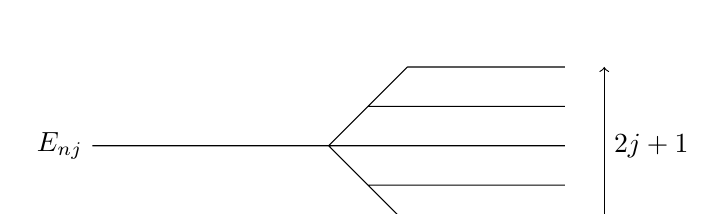
\begin{tikzpicture}
  \draw (0,0) node[left]{$E_{nj}$} -- (6,0)  (3,0) -- (4,1) (3,0) -- (4,-1)
        (4,1) -- (6,1) (3.5,0.5) -- (6,0.5) (3.5,-0.5) -- (6,-0.5) (4,-1) -- (6,-1);
  \draw[<->] (6.5,1) -- node[right]{$2j+1$} (6.5,-1);
\end{tikzpicture}
\par\end{center}

``Splitting'' of the ``multiplett''.

\noindent \begin{center}
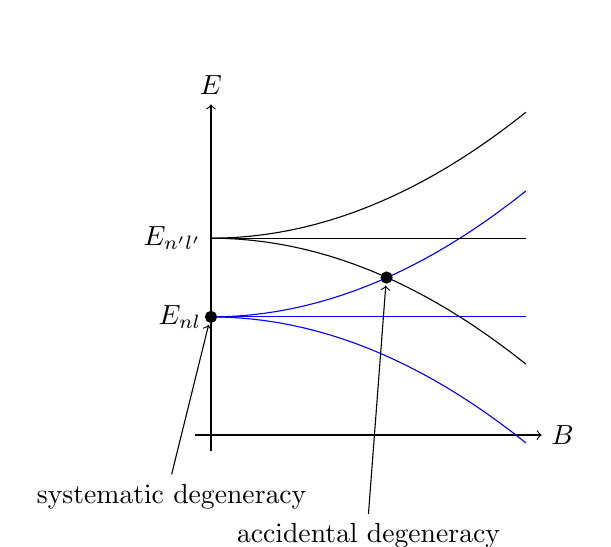
\begin{tikzpicture}[domain=0:4]
  \draw[->] (-0.2,0) -- (4.2,0) node[right] {$B$};
  \draw[->] (0,-0.2) -- (0,4.2) node[above] {$E$};
  \draw[color=blue] plot (\x,{0.1*(\x)^2+1.5});
  \draw[color=blue] plot (\x,{-0.1*(\x)^2+1.5});
  \draw[color=blue] plot (\x,1.5);
  \draw plot (\x,{0.1*(\x)^2+2.5});
  \draw plot (\x,{-0.1*(\x)^2+2.5});
  \draw plot (\x,2.5);
  \node at (0,1.5) [left] {$E_{nl}$};
  \node at (0,2.5) [left] {$E_{n'l'}$};
  \draw[->] (-0.5,-0.5) node[below]{systematic degeneracy} -- (-0.03,1.4);
  \draw[->] (2,-1) node[below]{accidental degeneracy} -- (2.22,1.9);
  \draw[fill=black] (2.23,2) circle (2pt);
  \draw[fill=black] (0,1.5) circle (2pt);
\end{tikzpicture} 
\par\end{center}


\subsection{Discrete symmetries}

You do not see them in classical mechanics.

\begin{iiilist}

\iii Parity inverts position and momentum vectors:
\begin{align*}
\hat{\pi}^{\dagger}\hat{q}_{i}\hat{\pi} & =-\hat{q}_{i}\\
\hat{\pi}^{\dagger}\hat{p}_{i}\hat{\pi} & =-\hat{p}_{i}
\end{align*}
But angular momentum doesn't change:
\begin{align*}
\hat{\pi}^{\dagger}\hat{j}_{i}\hat{\pi} & =\hat{j}_{i}
\end{align*}
These are called ``pseudo-vectors''.

States:
\begin{align*}
\hat{\pi}\KET{\vec{q}} & =\KET{-\vec{q}}\\
\hat{\pi}\KET{\vec{p}} & =\KET{-\vec{p}}
\end{align*}
\begin{align*}
\hat{\pi}^{2} & =\hat{I} & \hat{\pi}^{\dagger} & =\hat{\pi}^{-1} & \hat{\pi}^{\dagger} & =\hat{\pi}
\end{align*}
From these properties follows, that the eigenvalues of $\pi$ are
$\pm1$.

A $+1$ eigenstate is called \emph{even} and a $-1$ eigenstate is
called \emph{odd under parity}.

If we have $\hat{\pi}\KET{\alpha_{\pm}}=\pm\KET{\alpha_{\pm}}$ with
$\psi_{\pm}\left(\vec{q}\right)=\left\langle \vec{q}|\alpha_{\pm}\right\rangle $
then we get:
\begin{align*}
\psi_{\pm}\left(\pm\vec{q}\right) & =\pm\psi_{\pm}\left(\vec{q}\right)
\end{align*}
Example: $\hat{p}\KET p=p\KET p$
\begin{align*}
\left\langle q|p\right\rangle  & =\frac{1}{\sqrt{2m}}e^{\frac{\ii}{\hbar}pq}
\end{align*}
They are \emph{not} eigenstates of $\hat{\pi}$.
\begin{align*}
\KET{\alpha_{\pm}} & :=\frac{1}{\sqrt{2}}\left(\KET{\vec{p}}\pm\KET{-\vec{p}}\right)
\end{align*}
\begin{align*}
\left\langle q|\alpha_{\pm}\right\rangle  & =\begin{cases}
\frac{1}{\sqrt{2}}\cos\left(\frac{1}{\hbar}pq\right)\\
\frac{1}{\sqrt{2}}\sin\left(\frac{1}{\hbar}pq\right)
\end{cases}
\end{align*}
Example: Eigenstates of a central force $\KET{n,l,m}$.

We know, $\left[\hat{\vec{L}},\hat{\pi}\right]=0$, so automatically
$\KET{n,l,m}$ has a well defined parity. This means:
\begin{align*}
\hat{\pi}\KET{n,l,m} & =\pm\KET{n,l,m}
\end{align*}
Do your job:
\begin{align*}
\left\langle \vec{q}|n,l,m\right\rangle  & =R_{nl}\left(r\right)Y_{l}^{m}\left(\theta,\varphi\right)
\end{align*}
Change $\vec{q}\to-\vec{q}$. In spherical coordinates $\left(r,\theta,\varphi\right)\to\left(r,\pi-\theta,\varphi+\pi\right)$.
Remember:
\begin{align*}
Y_{l}^{m}\left(\theta,\varphi\right) & =\left(-1\right)^{m}\sqrt{\frac{\left(2l+1\right)\left(l-m\right)!}{4\pi\left(l+m\right)!}}\cdot P_{l}^{m}\left(\cos\theta\right)e^{\ii m\varphi}\\
Y_{l}^{m}\left(\pi-\theta,\varphi+\pi\right) & =\left(-1\right)^{l}Y_{l}^{m}\left(\theta,\varphi\right)
\end{align*}
Tips to construct $\hat{\pi}$.

1D harmonic oscillator:
\begin{align*}
\hat{H} & =\frac{1}{2m}\hat{p}^{2}+\frac{m\omega_{0}^{2}}{2}\hat{q}^{2}
\end{align*}
Check as an exercise:
\begin{align*}
\hat{\pi} & =e^{\ii\pi\hat{n}}
\end{align*}


Theorem:

If $\hat{H}\KET{e_{n}}=e_{n}\KET{e_{n}}$ and $\left[\hat{H},\hat{\pi}\right]=0$.
If the spectrum $e_{n}$ is \emph{not} degenerate, the eigenstates
of $\hat{H}$ have well defined parity.

\end{iiilist}


\chapter{Perturbation theory (time-independent)}


\chapter{Perturbation theory (time-dependent)}


\chapter{Many-particle systems}


\chapter{Scattering theory}


\chapter{Orthogonal Polynomials}

Sturm-Liouville equations:

Take $x\in\left[x_{0},x_{1}\right]$ and $a\left(x\right)\not=0$
and $a\left(x\right),b\left(x\right),c\left(x\right)\in C^{0}\left(\left[x_{0},x_{1}\right],\mathbb{R}\right)$:
\begin{align*}
a\left(x\right)\frac{\dd^{2}}{\dd x^{2}}y\left(x\right)+b\left(x\right)\frac{\dd}{\dd x}y\left(x\right)+c\left(x\right)y\left(x\right)+\lambda y\left(x\right) & =0
\end{align*}
Boundary condition:
\begin{align*}
\left[\alpha_{1}y\left(x\right)+\alpha_{2}\frac{\dd}{\dd x}y\left(x\right)\right]_{x=x_{0}} & =0\\
\left[\beta_{1}y\left(x\right)+\beta_{2}\frac{\dd}{\dd x}y\left(x\right)\right]_{x=x_{1}} & =0
\end{align*}
Define
\begin{align*}
p\left(x\right) & :=\exp\left(\int_{x_{0}}^{x}\frac{b\left(s\right)}{a\left(s\right)}\dd s\right)\\
r\left(x\right) & :=\frac{1}{a\left(x\right)}p\left(x\right)\\
q\left(x\right) & :=\frac{c\left(x\right)}{a\left(x\right)}p\left(x\right)
\end{align*}
to get:
\begin{align*}
\frac{\dd}{\dd x}\left(p\left(x\right)\frac{\dd}{\dd x}y\left(x\right)\right)+\left(q\left(x\right)+\lambda r\left(x\right)\right)y\left(x\right) & =0
\end{align*}
\begin{align*}
\hat{\mathscr{L}} & :=\frac{1}{r\left(x\right)}\left(\frac{\dd}{\dd x}\left(p\left(x\right)\frac{\dd}{\dd x}\right)+q\left(x\right)\right)
\end{align*}
\begin{align*}
\hat{\mathscr{L}}y_{n}\left(x\right) & =-\lambda_{n}y_{n}\left(x\right)
\end{align*}
This equation is solved by non-zero functions $y_{n}\left(x\right)$
for some $\lambda_{n}$.

Theorem: If $p\left(x\right)>0,r\left(x\right)>0$ and $q\left(x\right)\ge0$,
then the set $\left\{ y_{n}\left(x\right)\right\} _{n=1}$ is orthogonal,
that is:
\begin{align*}
\left\langle y_{n}|y_{m}\right\rangle :=\int_{x_{0}}^{x_{1}}r\left(x\right)y_{n}\left(x\right)y_{m}\left(x\right)\dd x & =k_{n}^{2}\delta_{nm}
\end{align*}
$r\left(x\right)$ is called ``weight''. Introduce a new set of
functions
\begin{align*}
\varphi_{n}\left(x\right) & :=y_{n}\left(x\right)\frac{\sqrt{r\left(x\right)}}{k_{n}}
\end{align*}
to get:
\begin{align*}
\int_{x_{0}}^{x_{1}}\varphi_{n}\left(x\right)\varphi_{m}\left(x\right)\dd x & =\delta_{nm}
\end{align*}
But the $\varphi_{n}\left(x\right)$ do not solve the differential
equation, so physicist don't use them.

\begin{iiilist}

\iii Legendre:
\begin{align*}
\underbrace{\left(1-x\right)^{2}}_{=a\left(x\right)}\frac{\dd^{2}y}{\dd x^{2}}\underbrace{-2x}_{=b\left(x\right)}\frac{\dd y}{\dd x}+\underbrace{n\left(n+1\right)}_{=\lambda}y & =0
\end{align*}
Defined for $x\in\left[-1,1\right]$. We get:
\begin{align*}
p\left(x\right) & =\exp\left(\int_{-1}^{x}\frac{-2s}{1-s^{2}}\dd s\right)=1-x^{2}\\
q\left(x\right) & =0\\
r\left(x\right) & =1
\end{align*}
This is the simplest value for $r\left(x\right)$.

Extra: The set $\left\{ 1,x,x^{2},\ldots,\right\} $ is linearly independent.
\begin{align*}
\int_{-1}^{1}r\left(x\right)x^{n}x^{m}\dd x & \not=\delta_{nm}
\end{align*}
Using the Gram-Schmidt-formalism to make orthogonal polynomials gives
for $r=1$ the Legendre polynomials.

In the Sturm-Liouville form:
\begin{align*}
\underbrace{\frac{\dd}{\dd x}\left(\left(1-x^{2}\right)\frac{\dd}{\dd x}\right)}_{=\hat{\mathscr{L}}}y\left(x\right) & =-n\left(n+1\right)y\left(x\right)
\end{align*}
Use power series and get normalized solutions:
\begin{align*}
p_{0}\left(x\right) & =1\\
p_{1}\left(x\right) & =x\\
p_{2}\left(x\right) & =\frac{1}{2}\left(3x^{2}-1\right)
\end{align*}
For each set of orthogonal polynomials there is a \emph{Rodrigues
formula}:
\begin{align*}
P_{n}\left(x\right) & =\frac{1}{2^{n}n!}\frac{\dd^{n}}{\dd x^{n}}\left(x^{2}-1\right)^{n}
\end{align*}
The \emph{recursion relation} is:
\begin{align*}
\left(n+1\right)P_{n+1}\left(x\right) & -\left(2n+1\right)xP_{n}\left(x\right)+nP_{n-1}\left(x\right)=0
\end{align*}
Every Sturm-Liouville equation solution satisfy a three term recursion
relation, because it is a second order equation.

The \emph{Generating function} is:
\begin{align*}
\frac{1}{\sqrt{1-2tz+t^{2}}} & =\sum_{n=0}^{\infty}t^{n}P_{n}\left(z\right)
\end{align*}


\iii Chebyshev:
\begin{align*}
\left(1-x^{2}\right)\frac{\dd^{2}y}{\dd x^{2}}-x\frac{\dd y}{\dd x}+\underbrace{n^{2}}_{=\lambda}y & =0
\end{align*}
for $x\in\left[-1,1\right]$.
\begin{align*}
p\left(x\right) & =\sqrt{1-x^{2}}\\
q\left(x\right) & =0\\
r\left(x\right) & =\frac{1}{\sqrt{1-x^{2}}}
\end{align*}
\begin{align*}
T_{0}\left(x\right) & =1\\
T_{1}\left(x\right) & =x\\
T_{2}\left(x\right) & =2x^{2}-1
\end{align*}
Rodrigues formula:
\begin{align*}
T_{n}\left(x\right) & =\cos\left(n\cos^{-1}\left(x\right)\right)
\end{align*}
What is the related potential in quantum mechanics?

\begin{align*}
\int_{-1}^{1}\frac{T_{n}\left(x\right)T_{m}\left(x\right)}{\sqrt{1-x^{2}}} & =\begin{cases}
\pi\delta_{nm} & n=0\\
\frac{\pi}{2}\delta_{nm} & n>0
\end{cases}
\end{align*}
Recursion:
\begin{align*}
T_{n+1}-2xT_{n}+T_{n-1} & =0
\end{align*}
Generating function:
\begin{align*}
\frac{1-t^{2}}{1-2tz+t^{2}} & =T_{0}\left(x\right)+2\sum_{n=1}^{\infty}T_{n}\left(x\right)t^{n}
\end{align*}


\iii Hermite:
\begin{align*}
\frac{\dd^{2}}{\dd x^{2}}y-2x\frac{\dd y}{\dd x}+\lambda y & =0
\end{align*}
We can take without trouble $x\in\left(-\infty,\infty\right)$.
\begin{align*}
p\left(x\right) & =e^{-x^{2}}\\
q\left(x\right) & =0\\
r\left(x\right) & =e^{-x^{2}}
\end{align*}
In Storm-Liouville form:
\begin{align*}
e^{x^{2}}\frac{\dd}{\dd x}\left(\left(e^{-x^{2}}\frac{\dd}{\dd x}\right)y\left(x\right)\right) & =-\lambda y\left(x\right)
\end{align*}
\begin{align*}
H_{0}\left(x\right) & =1\\
H_{1}\left(x\right) & =2x\\
H_{2}\left(x\right) & =4x^{2}-2
\end{align*}
Rodrigues formula:
\begin{align*}
H_{n}\left(x\right) & =\left(-1\right)^{n}e^{x^{2}}\frac{\dd^{n}}{\dd x^{n}}e^{-x^{2}}
\end{align*}
\begin{align*}
\int_{-\infty}^{\infty}e^{-x^{2}}H_{n}\left(x\right)H_{m}\left(x\right)\dd x & =2^{n}n!\sqrt{\pi}\delta_{nm}
\end{align*}
Recursion:
\begin{align*}
H_{n+1}-2xH_{n}+2nH_{n-1} & =0
\end{align*}
Generating function:
\begin{align*}
e^{-t^{2}+2tx} & =\sum_{n=0}^{\infty}\frac{t^{n}}{n!}H_{n}\left(x\right)
\end{align*}


\end{iiilist}


\part*{Appendix\thispagestyle{empty}}

\addcontentsline{toc}{part}{Appendix}

\fancyhead[R]{}
\fancyhead[C]{Appendix}


\chapter*{Acknowledgements}

\addcontentsline{toc}{section}{\hspace*{2.7em}Danksagungen}

\fancyhead[R]{Danksagungen}

My special thanks goes to Doctor Urbina, who gave this lecture and
allowed me to publish this script of the lecture.

I would also like to thank all those, who found errors by careful
reading and told me of them.

\vspace{1cm}


\hfill{}Andreas V�lklein


\chapter*{GNU Free Documentation License}

\addcontentsline{toc}{section}{\hspace*{2.7em}GNU Free Documentation License}

\fancyhead[R]{GNU Free Documentation License}

\noindent \begin{center}
Version 1.3, 3 November 2008\\
Copyright � 2000, 2001, 2002, 2007, 2008 Free Software Foundation,
Inc. 
\par\end{center}

\noindent \begin{center}
\texttt{<}\url{https://fsf.org/}\texttt{>}
\par\end{center}

\noindent \begin{center}
Everyone is permitted to copy and distribute verbatim copies of this
license document,\\
but changing it is not allowed
\par\end{center}


\section*{\noun{0. Preamble}}

\noindent The purpose of this License is to make a manual, textbook,
or other functional and useful document \textquotedblleft{}free\textquotedblright{}
in the sense of freedom: to assure everyone the effective freedom
to copy and redistribute it, with or without modifying it, either
commercially or noncommercially. Secondarily, this License preserves
for the author and publisher a way to get credit for their work, while
not being considered responsible for modifications made by others.

\noindent This License is a kind of \textquotedblleft{}copyleft\textquotedblright{},
which means that derivative works of the document must themselves
be free in the same sense. It complements the GNU General Public License,
which is a copyleft license designed for free software.

\noindent We have designed this License in order to use it for manuals
for free software, because free software needs free documentation:
a free program should come with manuals providing the same freedoms
that the software does. But this License is not limited to software
manuals; it can be used for any textual work, regardless of subject
matter or whether it is published as a printed book. We recommend
this License principally for works whose purpose is instruction or
reference.


\section*{\noun{1. Applicability and definitions}}

This License applies to any manual or other work, in any medium, that
contains a notice placed by the copyright holder saying it can be
distributed under the terms of this License. Such a notice grants
a world-wide, royalty-free license, unlimited in duration, to use
that work under the conditions stated herein. The \textquotedblleft{}\textbf{Document}\textquotedblright{},
below, refers to any such manual or work. Any member of the public
is a licensee, and is addressed as \textquotedblleft{}\textbf{you}\textquotedblright{}.
You accept the license if you copy, modify or distribute the work
in a way requiring permission under copyright law.

A \textquotedblleft{}\textbf{Modified Version}\textquotedblright{}
of the Document means any work containing the Document or a portion
of it, either copied verbatim, or with modifications and/or translated
into another language.

A \textquotedblleft{}\textbf{Secondary Section}\textquotedblright{}
is a named appendix or a front-matter section of the Document that
deals exclusively with the relationship of the publishers or authors
of the Document to the Document's overall subject (or to related matters)
and contains nothing that could fall directly within that overall
subject. (Thus, if the Document is in part a textbook of mathematics,
a Secondary Section may not explain any mathematics.) The relationship
could be a matter of historical connection with the subject or with
related matters, or of legal, commercial, philosophical, ethical or
political position regarding them.

The \textquotedblleft{}\textbf{Invariant Sections}\textquotedblright{}
are certain Secondary Sections whose titles are designated, as being
those of Invariant Sections, in the notice that says that the Document
is released under this License. If a section does not fit the above
definition of Secondary then it is not allowed to be designated as
Invariant. The Document may contain zero Invariant Sections. If the
Document does not identify any Invariant Sections then there are none.

The \textquotedblleft{}\textbf{Cover Texts}\textquotedblright{} are
certain short passages of text that are listed, as Front-Cover Texts
or Back-Cover Texts, in the notice that says that the Document is
released under this License. A Front-Cover Text may be at most 5 words,
and a Back-Cover Text may be at most 25 words.

A \textquotedblleft{}\textbf{Transparent}\textquotedblright{} copy
of the Document means a machine-readable copy, represented in a format
whose specification is available to the general public, that is suitable
for revising the document straightforwardly with generic text editors
or (for images composed of pixels) generic paint programs or (for
drawings) some widely available drawing editor, and that is suitable
for input to text formatters or for automatic translation to a variety
of formats suitable for input to text formatters. A copy made in an
otherwise Transparent file format whose markup, or absence of markup,
has been arranged to thwart or discourage subsequent modification
by readers is not Transparent. An image format is not Transparent
if used for any substantial amount of text. A copy that is not \textquotedblleft{}Transparent\textquotedblright{}
is called \textquotedblleft{}\textbf{Opaque}\textquotedblright{}.

Examples of suitable formats for Transparent copies include plain
ASCII without markup, Texinfo input format, \LaTeX{} input format,
SGML or XML using a publicly available DTD, and standard-conforming
simple HTML, PostScript or PDF designed for human modification. Examples
of transparent image formats include PNG, XCF and JPG. Opaque formats
include proprietary formats that can be read and edited only by proprietary
word processors, SGML or XML for which the DTD and/or processing tools
are not generally available, and the machine-generated HTML, PostScript
or PDF produced by some word processors for output purposes only.

The \textquotedblleft{}\textbf{Title Page}\textquotedblright{} means,
for a printed book, the title page itself, plus such following pages
as are needed to hold, legibly, the material this License requires
to appear in the title page. For works in formats which do not have
any title page as such, \textquotedblleft{}Title Page\textquotedblright{}
means the text near the most prominent appearance of the work's title,
preceding the beginning of the body of the text.

The \textquotedblleft{}\textbf{publisher}\textquotedblright{} means
any person or entity that distributes copies of the Document to the
public.

A section \textquotedblleft{}\textbf{Entitled XYZ}\textquotedblright{}
means a named subunit of the Document whose title either is precisely
XYZ or contains XYZ in parentheses following text that translates
XYZ in another language. (Here XYZ stands for a specific section name
mentioned below, such as \textquotedblleft{}\textbf{Acknowledgements}\textquotedblright{},
\textquotedblleft{}\textbf{Dedications}\textquotedblright{}, \textquotedblleft{}\textbf{Endorsements}\textquotedblright{},
or \textquotedblleft{}\textbf{History}\textquotedblright{}.) To \textquotedblleft{}\textbf{Preserve
the Title}\textquotedblright{} of such a section when you modify the
Document means that it remains a section \textquotedblleft{}Entitled
XYZ\textquotedblright{} according to this definition.

The Document may include Warranty Disclaimers next to the notice which
states that this License applies to the Document. These Warranty Disclaimers
are considered to be included by reference in this License, but only
as regards disclaiming warranties: any other implication that these
Warranty Disclaimers may have is void and has no effect on the meaning
of this License.


\section*{\noun{2. Verbatim copying}}

You may copy and distribute the Document in any medium, either commercially
or noncommercially, provided that this License, the copyright notices,
and the license notice saying this License applies to the Document
are reproduced in all copies, and that you add no other conditions
whatsoever to those of this License. You may not use technical measures
to obstruct or control the reading or further copying of the copies
you make or distribute. However, you may accept compensation in exchange
for copies. If you distribute a large enough number of copies you
must also follow the conditions in section 3.

You may also lend copies, under the same conditions stated above,
and you may publicly display copies.


\section*{\noun{3. Copying in quantity}}

If you publish printed copies (or copies in media that commonly have
printed covers) of the Document, numbering more than 100, and the
Document's license notice requires Cover Texts, you must enclose the
copies in covers that carry, clearly and legibly, all these Cover
Texts: Front-Cover Texts on the front cover, and Back-Cover Texts
on the back cover. Both covers must also clearly and legibly identify
you as the publisher of these copies. The front cover must present
the full title with all words of the title equally prominent and visible.
You may add other material on the covers in addition. Copying with
changes limited to the covers, as long as they preserve the title
of the Document and satisfy these conditions, can be treated as verbatim
copying in other respects.

If the required texts for either cover are too voluminous to fit legibly,
you should put the first ones listed (as many as fit reasonably) on
the actual cover, and continue the rest onto adjacent pages.

If you publish or distribute Opaque copies of the Document numbering
more than 100, you must either include a machine-readable Transparent
copy along with each Opaque copy, or state in or with each Opaque
copy a computer-network location from which the general network-using
public has access to download using public-standard network protocols
a complete Transparent copy of the Document, free of added material.
If you use the latter option, you must take reasonably prudent steps,
when you begin distribution of Opaque copies in quantity, to ensure
that this Transparent copy will remain thus accessible at the stated
location until at least one year after the last time you distribute
an Opaque copy (directly or through your agents or retailers) of that
edition to the public.

It is requested, but not required, that you contact the authors of
the Document well before redistributing any large number of copies,
to give them a chance to provide you with an updated version of the
Document.


\section*{\noun{4. Modifications}}

You may copy and distribute a Modified Version of the Document under
the conditions of sections 2 and 3 above, provided that you release
the Modified Version under precisely this License, with the Modified
Version filling the role of the Document, thus licensing distribution
and modification of the Modified Version to whoever possesses a copy
of it. In addition, you must do these things in the Modified Version:
\begin{description}
\item [{A.\hspace*{3.2mm}}] Use in the Title Page (and on the covers,
if any) a title distinct from that of the Document, and from those
of previous versions (which should, if there were any, be listed in
the History section of the Document). You may use the same title as
a previous version if the original publisher of that version gives
permission.
\item [{B.\hspace*{3.4mm}}] List on the Title Page, as authors, one or
more persons or entities responsible for authorship of the modifications
in the Modified Version, together with at least five of the principal
authors of the Document (all of its principal authors, if it has fewer
than five), unless they release you from this requirement.
\item [{C.\hspace*{3.4mm}}] State on the Title page the name of the publisher
of the Modified Version, as the publisher.
\item [{D.\hspace*{3.4mm}}] Preserve all the copyright notices of the
Document.
\item [{E.\hspace*{3.4mm}}] Add an appropriate copyright notice for your
modifications adjacent to the other copyright notices.
\item [{F.\hspace*{3.8mm}}] Include, immediately after the copyright notices,
a license notice giving the public permission to use the Modified
Version under the terms of this License, in the form shown in the
Addendum below.
\item [{G.\hspace*{3.1mm}}] Preserve in that license notice the full lists
of Invariant Sections and required Cover Texts given in the Document's
license notice.
\item [{H.\hspace*{3.2mm}}] Include an unaltered copy of this License.
\item [{I.\hspace*{5.0mm}}] Preserve the section Entitled \textquotedblleft{}History\textquotedblright{},
Preserve its Title, and add to it an item stating at least the title,
year, new authors, and publisher of the Modified Version as given
on the Title Page. If there is no section Entitled \textquotedblleft{}History\textquotedblright{}
in the Document, create one stating the title, year, authors, and
publisher of the Document as given on its Title Page, then add an
item describing the Modified Version as stated in the previous sentence.
\item [{J.\hspace*{4.3mm}}] Preserve the network location, if any, given
in the Document for public access to a Transparent copy of the Document,
and likewise the network locations given in the Document for previous
versions it was based on. These may be placed in the \textquotedblleft{}History\textquotedblright{}
section. You may omit a network location for a work that was published
at least four years before the Document itself, or if the original
publisher of the version it refers to gives permission.
\item [{K.\hspace*{3.3mm}}] For any section Entitled \textquotedblleft{}Acknowledgements\textquotedblright{}
or \textquotedblleft{}Dedications\textquotedblright{}, Preserve the
Title of the section, and preserve in the section all the substance
and tone of each of the contributor acknowledgements and/or dedications
given therein.
\item [{L.\hspace*{4.1mm}}] Preserve all the Invariant Sections of the
Document, unaltered in their text and in their titles. Section numbers
or the equivalent are not considered part of the section titles.
\item [{M.\hspace*{3mm}}] Delete any section Entitled \textquotedblleft{}Endorsements\textquotedblright{}.
Such a section may not be included in the Modified Version.
\item [{N.\hspace*{3.4mm}}] Do not retitle any existing section to be
Entitled \textquotedblleft{}Endorsements\textquotedblright{} or to
conflict in title with any Invariant Section.
\item [{O.\hspace*{3.4mm}}] Preserve any Warranty Disclaimers.
\end{description}
If the Modified Version includes new front-matter sections or appendices
that qualify as Secondary Sections and contain no material copied
from the Document, you may at your option designate some or all of
these sections as invariant. To do this, add their titles to the list
of Invariant Sections in the Modified Version's license notice. These
titles must be distinct from any other section titles.

You may add a section Entitled \textquotedblleft{}Endorsements\textquotedblright{},
provided it contains nothing but endorsements of your Modified Version
by various parties\textemdash{}for example, statements of peer review
or that the text has been approved by an organization as the authoritative
definition of a standard.

You may add a passage of up to five words as a Front-Cover Text, and
a passage of up to 25 words as a Back-Cover Text, to the end of the
list of Cover Texts in the Modified Version. Only one passage of Front-Cover
Text and one of Back-Cover Text may be added by (or through arrangements
made by) any one entity. If the Document already includes a cover
text for the same cover, previously added by you or by arrangement
made by the same entity you are acting on behalf of, you may not add
another; but you may replace the old one, on explicit permission from
the previous publisher that added the old one.

The author(s) and publisher(s) of the Document do not by this License
give permission to use their names for publicity for or to assert
or imply endorsement of any Modified Version.


\section*{\noun{5. Combining documents}}

You may combine the Document with other documents released under this
License, under the terms defined in section 4 above for modified versions,
provided that you include in the combination all of the Invariant
Sections of all of the original documents, unmodified, and list them
all as Invariant Sections of your combined work in its license notice,
and that you preserve all their Warranty Disclaimers.

The combined work need only contain one copy of this License, and
multiple identical Invariant Sections may be replaced with a single
copy. If there are multiple Invariant Sections with the same name
but different contents, make the title of each such section unique
by adding at the end of it, in parentheses, the name of the original
author or publisher of that section if known, or else a unique number.
Make the same adjustment to the section titles in the list of Invariant
Sections in the license notice of the combined work.

In the combination, you must combine any sections Entitled \textquotedblleft{}History\textquotedblright{}
in the various original documents, forming one section Entitled \textquotedblleft{}History\textquotedblright{};
likewise combine any sections Entitled \textquotedblleft{}Acknowledgements\textquotedblright{},
and any sections Entitled \textquotedblleft{}Dedications\textquotedblright{}.
You must delete all sections Entitled \textquotedblleft{}Endorsements\textquotedblright{}.


\section*{\noun{6. Collections of documents}}

You may make a collection consisting of the Document and other documents
released under this License, and replace the individual copies of
this License in the various documents with a single copy that is included
in the collection, provided that you follow the rules of this License
for verbatim copying of each of the documents in all other respects.

You may extract a single document from such a collection, and distribute
it individually under this License, provided you insert a copy of
this License into the extracted document, and follow this License
in all other respects regarding verbatim copying of that document.


\section*{\noun{7. Aggregation with independent works}}

A compilation of the Document or its derivatives with other separate
and independent documents or works, in or on a volume of a storage
or distribution medium, is called an \textquotedblleft{}aggregate\textquotedblright{}
if the copyright resulting from the compilation is not used to limit
the legal rights of the compilation's users beyond what the individual
works permit. When the Document is included in an aggregate, this
License does not apply to the other works in the aggregate which are
not themselves derivative works of the Document.

If the Cover Text requirement of section 3 is applicable to these
copies of the Document, then if the Document is less than one half
of the entire aggregate, the Document's Cover Texts may be placed
on covers that bracket the Document within the aggregate, or the electronic
equivalent of covers if the Document is in electronic form. Otherwise
they must appear on printed covers that bracket the whole aggregate.


\section*{\noun{8. Translation}}

Translation is considered a kind of modification, so you may distribute
translations of the Document under the terms of section 4. Replacing
Invariant Sections with translations requires special permission from
their copyright holders, but you may include translations of some
or all Invariant Sections in addition to the original versions of
these Invariant Sections. You may include a translation of this License,
and all the license notices in the Document, and any Warranty Disclaimers,
provided that you also include the original English version of this
License and the original versions of those notices and disclaimers.
In case of a disagreement between the translation and the original
version of this License or a notice or disclaimer, the original version
will prevail.

If a section in the Document is Entitled \textquotedblleft{}Acknowledgements\textquotedblright{},
\textquotedblleft{}Dedications\textquotedblright{}, or \textquotedblleft{}History\textquotedblright{},
the requirement (section 4) to Preserve its Title (section 1) will
typically require changing the actual title.


\section*{\noun{9. Termination}}

You may not copy, modify, sublicense, or distribute the Document except
as expressly provided under this License. Any attempt otherwise to
copy, modify, sublicense, or distribute it is void, and will automatically
terminate your rights under this License.

However, if you cease all violation of this License, then your license
from a particular copyright holder is reinstated (a) provisionally,
unless and until the copyright holder explicitly and finally terminates
your license, and (b) permanently, if the copyright holder fails to
notify you of the violation by some reasonable means prior to 60 days
after the cessation.

Moreover, your license from a particular copyright holder is reinstated
permanently if the copyright holder notifies you of the violation
by some reasonable means, this is the first time you have received
notice of violation of this License (for any work) from that copyright
holder, and you cure the violation prior to 30 days after your receipt
of the notice.

Termination of your rights under this section does not terminate the
licenses of parties who have received copies or rights from you under
this License. If your rights have been terminated and not permanently
reinstated, receipt of a copy of some or all of the same material
does not give you any rights to use it.


\section*{\noun{10. Future revisions of this license}}

The Free Software Foundation may publish new, revised versions of
the GNU Free Documentation License from time to time. Such new versions
will be similar in spirit to the present version, but may differ in
detail to address new problems or concerns. See \url{https://www.gnu.org/copyleft/}.

Each version of the License is given a distinguishing version number.
If the Document specifies that a particular numbered version of this
License \textquotedbl{}or any later version\textquotedbl{} applies
to it, you have the option of following the terms and conditions either
of that specified version or of any later version that has been published
(not as a draft) by the Free Software Foundation. If the Document
does not specify a version number of this License, you may choose
any version ever published (not as a draft) by the Free Software Foundation.
If the Document specifies that a proxy can decide which future versions
of this License can be used, that proxy's public statement of acceptance
of a version permanently authorizes you to choose that version for
the Document.


\section*{\noun{11. Relicensing}}

\textquotedblleft{}Massive Multiauthor Collaboration Site\textquotedblright{}
(or \textquotedblleft{}MMC Site\textquotedblright{}) means any World
Wide Web server that publishes copyrightable works and also provides
prominent facilities for anybody to edit those works. A public wiki
that anybody can edit is an example of such a server. A \textquotedblleft{}Massive
Multiauthor Collaboration\textquotedblright{} (or \textquotedblleft{}MMC\textquotedblright{})
contained in the site means any set of copyrightable works thus published
on the MMC site.

\textquotedblleft{}CC-BY-SA\textquotedblright{} means the Creative
Commons Attribution-Share Alike 3.0 license published by Creative
Commons Corporation, a not-for-profit corporation with a principal
place of business in San Francisco, California, as well as future
copyleft versions of that license published by that same organization.

\textquotedblleft{}Incorporate\textquotedblright{} means to publish
or republish a Document, in whole or in part, as part of another Document.

An MMC is \textquotedblleft{}eligible for relicensing\textquotedblright{}
if it is licensed under this License, and if all works that were first
published under this License somewhere other than this MMC, and subsequently
incorporated in whole or in part into the MMC, (1) had no cover texts
or invariant sections, and (2) were thus incorporated prior to November
1, 2008.

The operator of an MMC Site may republish an MMC contained in the
site under CC-BY-SA on the same site at any time before August 1,
2009, provided the MMC is eligible for relicensing.


\section*{\noun{Addendum}: How to use this License for your documents}

To use this License in a document you have written, include a copy
of the License in the document and put the following copyright and
license notices just after the title page:
\begin{quote}
Copyright � YEAR YOUR NAME.\\
Permission is granted to copy, distribute and/or modify this document
under the terms of the GNU Free Documentation License, Version 1.3
or any later version published by the Free Software Foundation;

with no Invariant Sections, no Front-Cover Texts, and no Back-Cover
Texts.

A copy of the license is included in the section entitled \textquotedbl{}GNU
Free Documentation License\textquotedbl{}.
\end{quote}
If you have Invariant Sections, Front-Cover Texts and Back-Cover Texts,
replace the \textquotedbl{}with $\ldots$ Texts.\textquotedbl{} line
with this:
\begin{quote}
with the Invariant Sections being LIST THEIR TITLES, with the Front-Cover
Texts being LIST, and with the Back-Cover Texts being LIST.
\end{quote}
If you have Invariant Sections without Cover Texts, or some other
combination of the three, merge those two alternatives to suit the
situation.

If your document contains nontrivial examples of program code, we
recommend releasing these examples in parallel under your choice of
free software license, such as the GNU General Public License, to
permit their use in free software.

\label{END}
\end{document}
